%%%%%%%%%%%%%%%%%%%%%%%%%%%%%%%%%%%%%%%%%
% Beamer Presentation
% LaTeX Template
% Version 1.0 (10/11/12)
%
% This template has been downloaded from:
% http://www.LaTeXTemplates.com
%
% License:
% CC BY-NC-SA 3.0 (http://creativecommons.org/licenses/by-nc-sa/3.0/)
%
%%%%%%%%%%%%%%%%%%%%%%%%%%%%%%%%%%%%%%%%%

%----------------------------------------------------------------------------------------
%	PACKAGES AND THEMES
%----------------------------------------------------------------------------------------

\documentclass{beamer}
\newcounter{saveenumi}
\newcommand{\seti}{\setcounter{saveenumi}{\value{enumi}}}
\newcommand{\conti}{\setcounter{enumi}{\value{saveenumi}}}
\mode<presentation> {

% The Beamer class comes with a number of default slide themes
% which change the colors and layouts of slides. Below this is a list
% of all the themes, uncomment each in turn to see what they look like.
\usepackage{bookman}
%\usetheme{default}
%\usetheme{AnnArbor}
%\usetheme{Antibes}
%\usetheme{Bergen}
%\usetheme{Berkeley}
%\usetheme{Berlin}
%\usetheme{Boadilla}
%\usetheme{CambridgeUS}
%\usetheme{Copenhagen}
%\usetheme{Darmstadt}
%\usetheme{Dresden}
%\usetheme{Frankfurt}
%\usetheme{Goettingen}
%\usetheme{Hannover}
%\usetheme{Ilmenau}
%\usetheme{JuanLesPins}
%\usetheme{Luebeck}
\usetheme{Madrid}
%\usetheme{Malmoe}
%\usetheme{Marburg}
%\usetheme{Montpellier}
%\usetheme{PaloAlto}
%\usetheme{Pittsburgh}
%\usetheme{Rochester}
%\usetheme{Singapore}
%\usetheme{Szeged}
%\usetheme{Warsaw}

% As well as themes, the Beamer class has a number of color themes
% for any slide theme. Uncomment each of these in turn to see how it
% changes the colors of your current slide theme.

%\usecolortheme{albatross}
%\usecolortheme{beaver}
%\usecolortheme{beetle}
%\usecolortheme{crane}
\usecolortheme{dolphin}
%\usecolortheme{dove}
%\usecolortheme{fly}
%\usecolortheme{lily}

%\usecolortheme{orchid}
%\usecolortheme{rose}
%\usecolortheme{seagull}
%\usecolortheme{seahorse}
%\usecolortheme{whale}
%\usecolortheme{wolverine}

%\setbeamertemplate{footline} % To remove the footer line in all slides uncomment this line
%\setbeamertemplate{footline}[page number] % To replace the footer line in all slides with a simple slide count uncomment this line

%\setbeamertemplate{navigation symbols}{} % To remove the navigation symbols from the bottom of all slides uncomment this line
}

\usepackage{graphicx} % Allows including images
\usepackage{mathrsfs}
\usepackage{booktabs} % Allows the use of \toprule, \midrule and \bottomrule in tables
\usepackage{amsmath}
%\usepackage{fontspec}


%\usepackage[demo]{graphicx}
%\usepackage{caption}
%\usepackage{subcaption}
%\usepackage{subfig}


%----------------------------------------------------------------------------------------
%	TITLE PAGE
%----------------------------------------------------------------------------------------

\title[Sun-Avoidance Slew (SAS) Maneuver ]{Sun-Avoidance Slew Planning Algorithm with Pointing and Actuator Constraints
\\(AAS 19-801) } % The short title appears at the bottom of every slide, the full title is only on the title page
\subtitle{}
\author[M. Ayoubi\ \& J. Hsin]{Mohammad. A. Ayoubi\inst{1} \and Junette Hsin\inst{2}}
%Maxar Space Solutions\\ (Formerly Space Systems/Loral)}
%\author[M. Ayoubi\ \& J. Hsin]{Mohammad. A. Ayoubi\inst{\dagger} \ and Junette Hsin \inst{2}}
%\institute[]{\inst[1]{Department of Mechanical Engineering} Associate Professor \and %
%                      \inst[2]{Dynamics and Control Analysis Group} Engineer}

%\institute[]{AIAA/AAS Astrodynamics Specialist Conference, Portland, ME\\
%11-- 15 August 2019}

\subtitle{AIAA/AAS Astrodynamics Specialist Conference,\\ Portland, ME, 11-- 15 August 2019}
\institute[]{\inst{1} Associate Professor, Department of Mechanical Engineering, Santa Clara University, \\ \inst{2} Engineer, Dynamics and Control Analysis Group, Maxar Space Infrastructure (Formerly Space Systems/Loral)}

\date{}		


\begin{document}
\begin{frame}
  \titlepage
\end{frame}

%-------------------------------------------------------------------------------------------------------------------------------------------------------------------
\begin{frame}{Outlines}
\begin{block}{}
\tableofcontents
\end{block}
\end{frame}
%-------------------------------------------------------------------------------------------------------------------------------------------------------------------
\begin{frame}
\section{Previous Literature}
\begin{block}{Introduction}
	The attitude reorientation problem in the presence of attitude constrained zones has been studied in the last three decades:
	\begin{enumerate} 
		
		\item McInnes (1994): artificial potential function. He proposed an entirely analytical guidance law which was suitable for onboard implementation. 
		\begin{enumerate}
			\item However, he used Euler angles, which are singular for large slew angles. 
		\end{enumerate}
		\item Spindle (1998), Hablani (1998), Biggs and Colley (2016), Frazzoli (2001): A geometric approach was proposed where a feasible attitude maneuver, or a guidance law, is precomputed based on the attitude-avoidance-zone constraints or randomized algorithms. 
		\begin{enumerate}
			\item However, depending on the number of constraints and initial and final attitudes, this approach can be computationally expensive and not suitable for onboard implementation. 
		\end{enumerate}
		
	\end{enumerate} 
\end{block}
\end{frame}
%-------------------------------------------------------------------------------------------------------------------------------------------------------------------
\section{Introduction}
\begin{frame}
		\begin{block}{Previous Literature}
			\begin{enumerate}
				\item Spiller (2016): Particle swarm optimization (PSO) technique to find a sub-optimal solution with keep-out constraints. 
				\item Another approach casted the problem as a convex optimization problem and used semi-definite programming (SDP) or quadratically constrained quadratic programming (QCQP) in its solution (see for instance Kim and Mesbahi, Kim et al., Sun and Dai, and Lee and Mesbahi.
				\item Recently, Ramos and Schaub proposed a method based on the Lyapunov stability theorem and logarithmic barrier potential function to derive a steering law for attitude control of a spacecraft subject to conically constrained inclusion and exclusion regions. They also considered the control-torque constraint in their algorithm.  
		\end{enumerate}
	\end{block}
\end{frame}
%-------------------------------------------------------------------------------------------------------------------------------------------------------------------
\begin{frame}
\begin{block}{SAS Algorithm}
	\begin{enumerate} 
		\item The SAS algorithm is a geometric approach for a sun (or any bright object) avoidance slew maneuver with pointing and actuator constraints. 
		\item Assumption: spacecraft has a single light-sensitive payload with control-torque and reaction wheels' angular momentum constraints
		\item Assumption: The initial and final attitudes, instrument boresight vector, and sun vector are known. 
		\item Pontryagin's minimum principle (PMP) is used to derive the desired or target-frame quaternions, angular velocity and acceleration for two cases: 
		\begin{enumerate}
			\item with control-torque and reaction wheels' angular momentum constraints
			\item with control-torque constraints
		\end{enumerate} 
		\item Numerical simulation is performed to show the viability of the proposed algorithm with control-torque and angular momentum constraints.
	\end{enumerate} 
\end{block}
\end{frame}
%%-------------------------------------------------------------------------------------------------------------------------------------------------------------------
\begin{frame}{Sun-Avoidance Slew (SAS) Algorithm}
\begin{block}{}
	\begin{figure}
		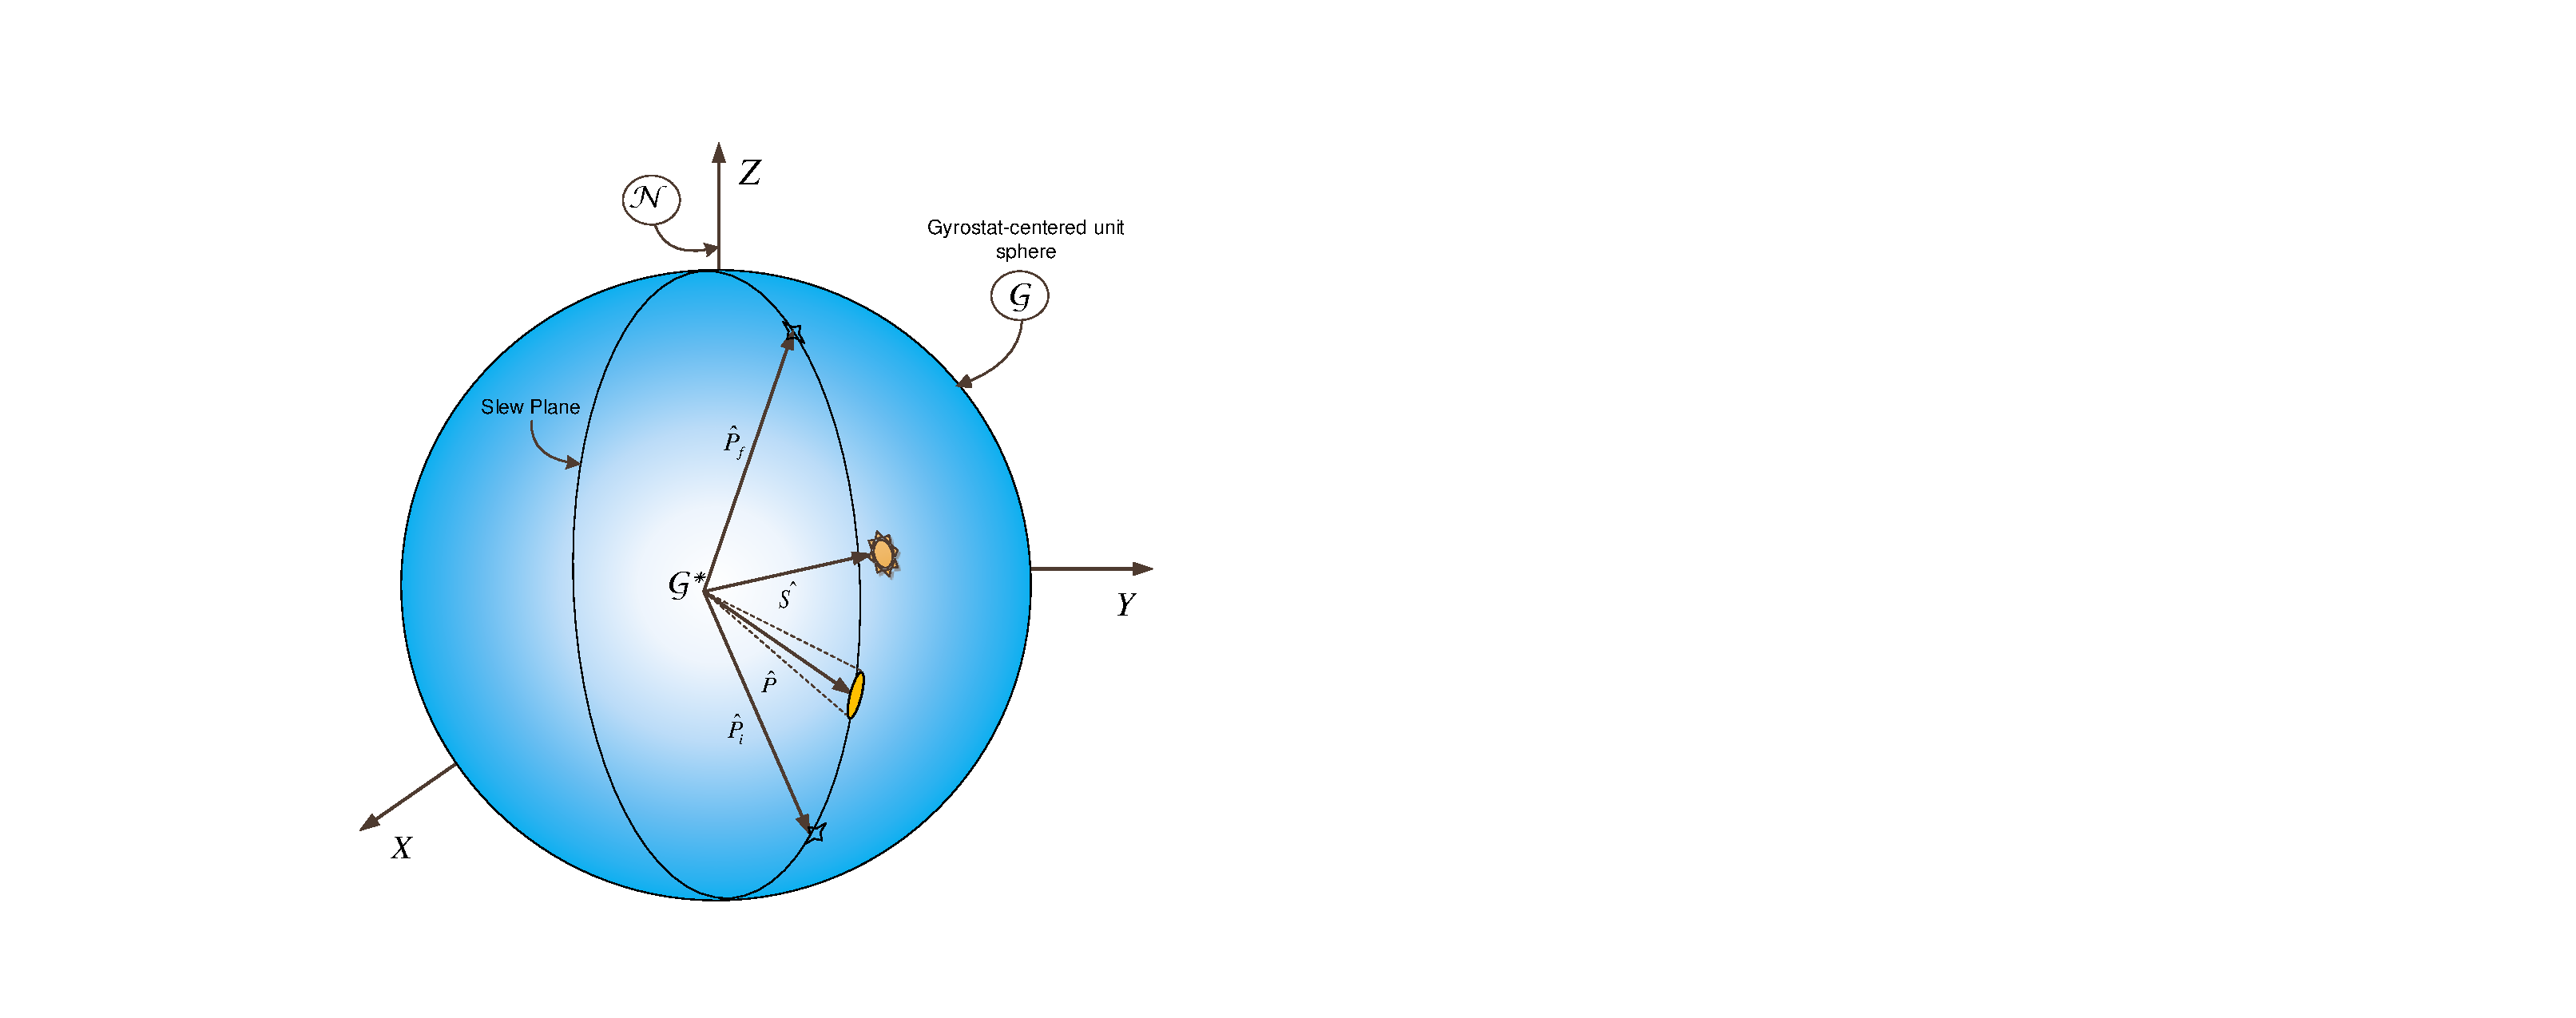
\includegraphics[width=3in]{./Figures/SASSchematic1}
		\caption{The gyrostat-centered unit sphere.}
	\end{figure}
\end{block}
\end{frame}
%-------------------------------------------------------------------------------------------------------------------------------------------------------------------
\section{Sun-Avoidance Slew (SAS) Algorithm}

\begin{frame}{Sun-Avoidance Slew (SAS) Algorithm}
	\begin{block}{Problem Statement:}
		Given:$_\mathcal{N}\hat{P}_i$, $_\mathcal{N}\hat{P}_f$, $_\mathcal{N}\hat{S}$, $_\mathcal{G}\hat{P}$, $\epsilon_p$, $^\mathcal{N}q^\mathcal{G}$, $^\mathcal{N}_\mathcal{G}\omega^\mathcal{G}(t_i)$, and $^\mathcal{N}_\mathcal{G}\omega^\mathcal{G}(t_f)$ .\\
		Assumption: The spacecraft is rigid.\\
		Find: 
		\begin{enumerate}
			\item A sequence of slew maneuvers to avoid sun vector.
			\item the commanded angular velocity, angular acceleration, and quaternion profiles.
		\end{enumerate} 
%		\begin{figure}
%			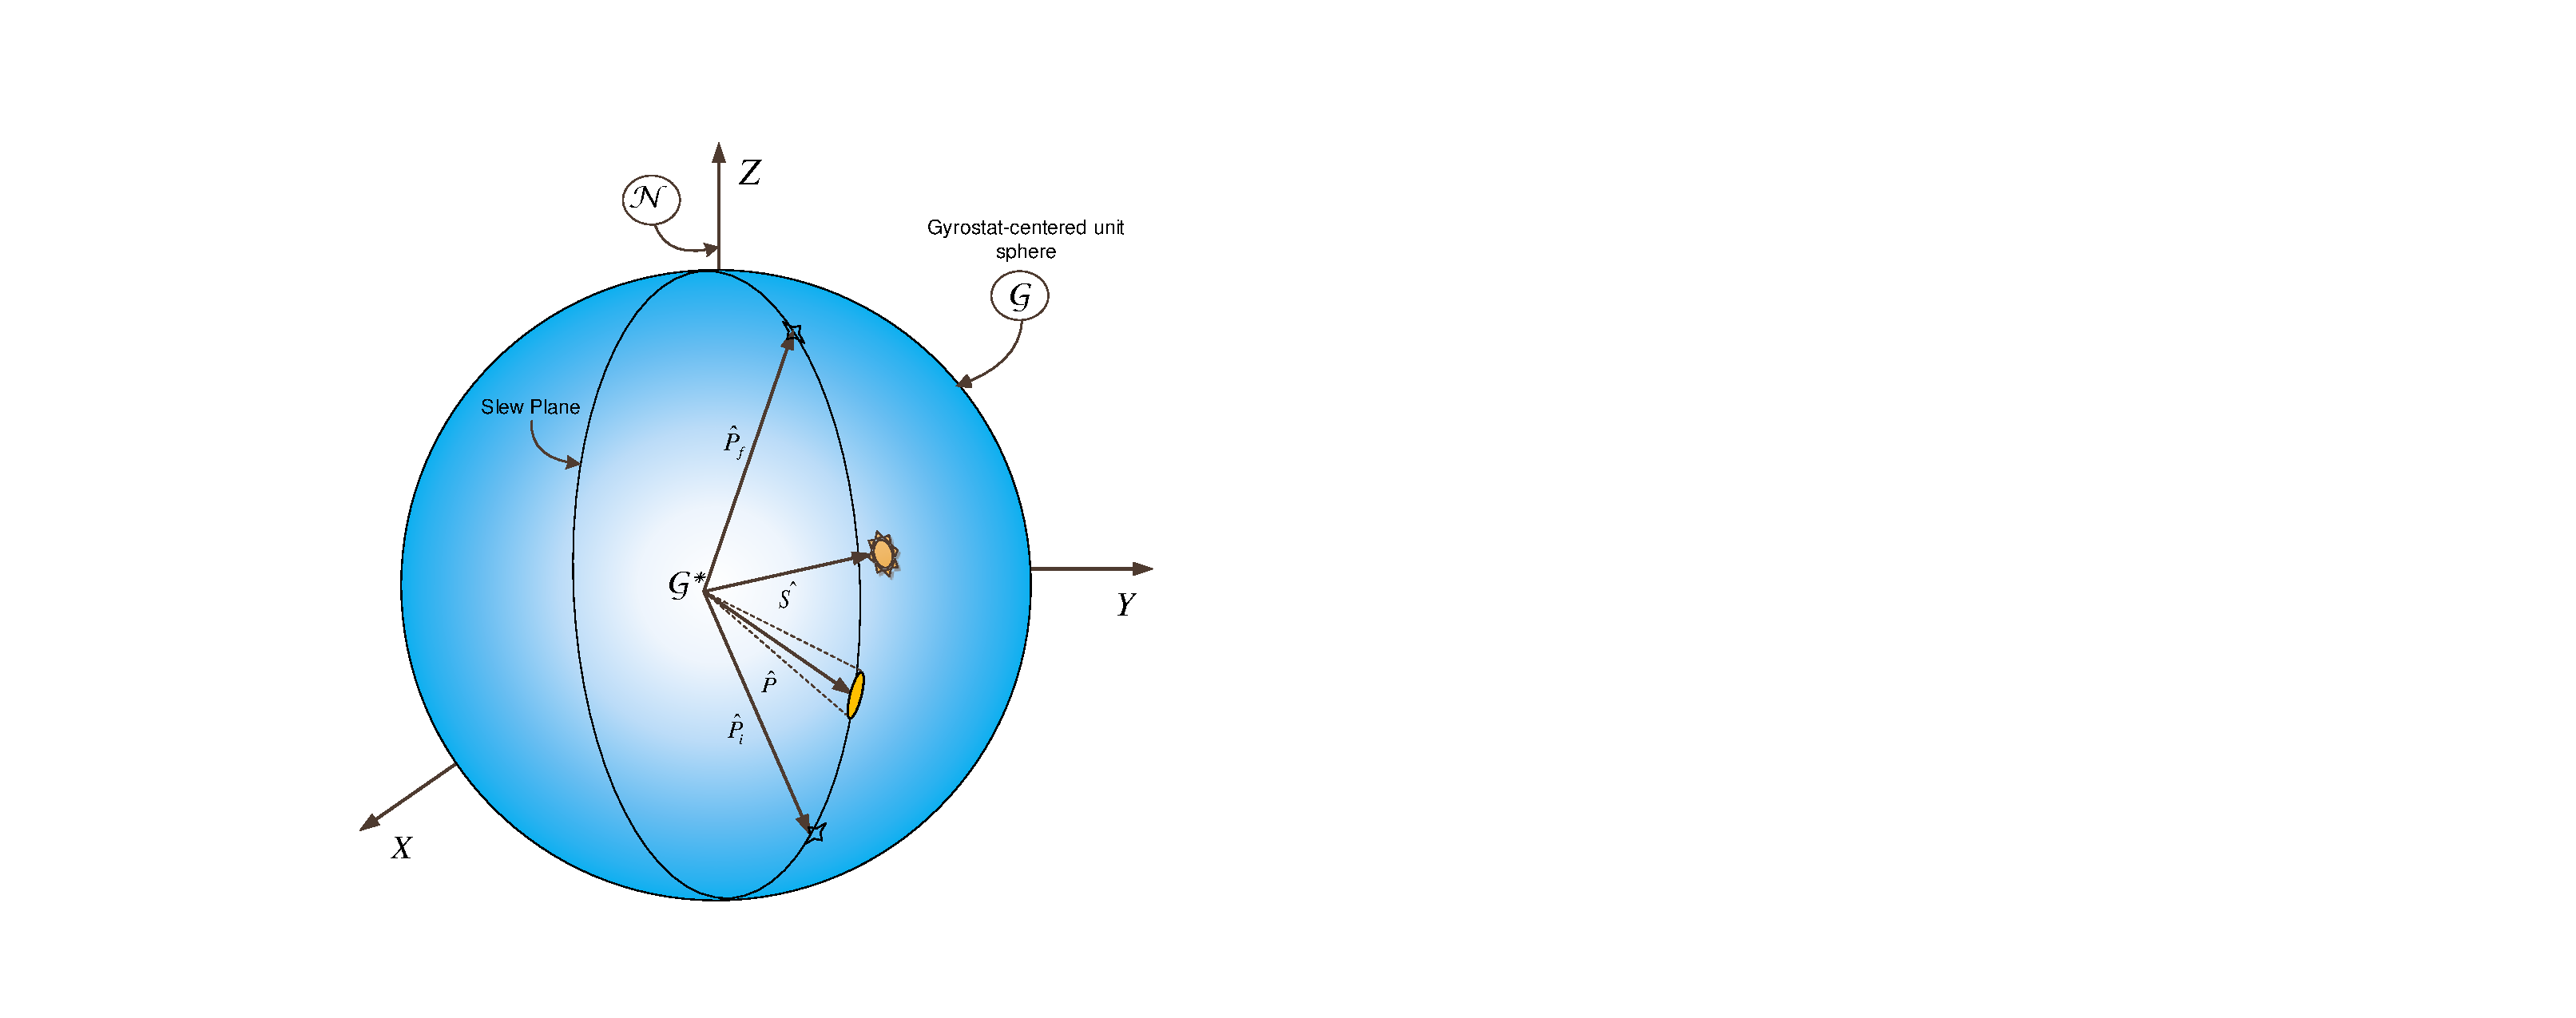
\includegraphics[width=1.5in]{./Figures/SASSchematic1}
%		\end{figure}
	\end{block}
\end{frame}
%%-------------------------------------------------------------------------------------------------------------------------------------------------------------------
%\begin{frame}{Sun-Avoidance Slew (SAS) Algorithm}
%\begin{block}{Nomenclature}
%\begin{itemize}
%\item $\mathcal{G}$ frame: Unit sphere attached to the gyrostat.
%\item $\mathcal{N}$: frame: The Newtonian frame fixed in the inertial space.
%\item $_\mathcal{G}\hat{P}$: Unit vector along the bore sight of payload in the $\mathcal{G}$ frame.
%\item $_\mathcal{G}\hat{P}_i$: Unit vector of the initial point in the $\mathcal{G}$ frame.
%\item $_\mathcal{G}\hat{P}_f$: Unit vector of the final point in the $\mathcal{G}$ frame.
%\item $_\mathcal{N}\hat{S}$: Unit vector of the sun vector in the $\mathcal{N}$ frame.
% \item $\epsilon_p$: Payload half-cone angle.
%\end{itemize}
%\end{block}
%\end{frame}
%%-------------------------------------------------------------------------------------------------------------------------------------------------------------------
\begin{frame}{Summary of the Algorithm}
\begin{block}{}
	\begin{figure}
		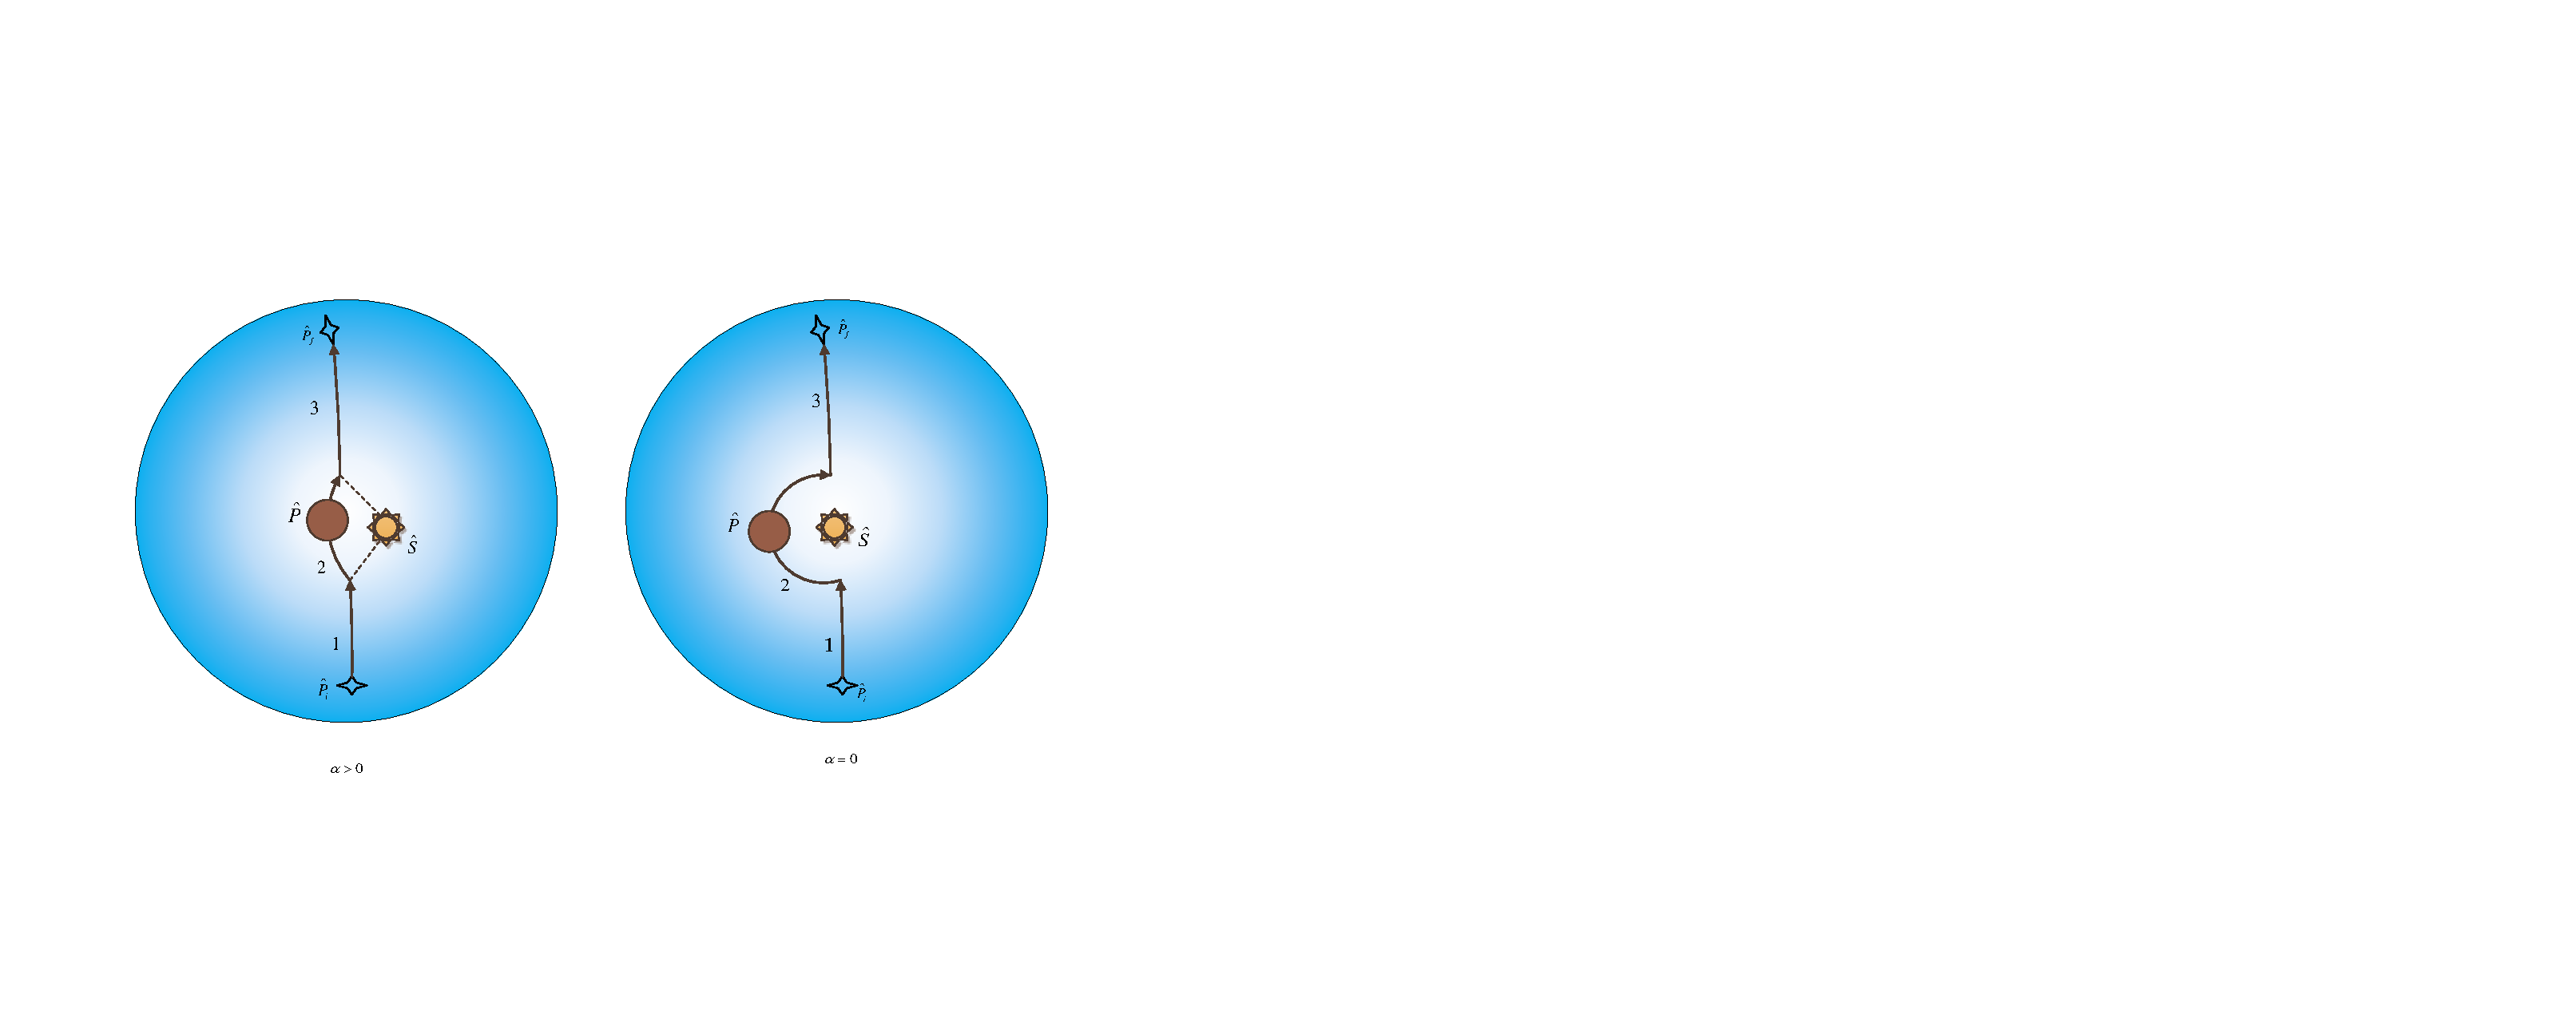
\includegraphics[width=4.85in]{./Figures/SASSchematic3}
	\end{figure}
\end{block}
\end{frame}
%
%%-------------------------------------------------------------------------------------------------------------------------------------------------------------------
\begin{frame}{Sun-Avoidance Slew (SAS) Algorithm}
\begin{block}{Check the Sun Vector Intrusion}
\begin{enumerate}
\item Check the angular separation, $\alpha$, between the sun vector, $\hat{S}$, and the $\hat{P}_i-\hat{P}_f$ or ``slew'' plane.
\begin{equation}
\alpha=\frac{\pi}{2}-\cos^{-1}(\hat{S}\cdot_\mathcal{N}\hat{e})
\end{equation}
where the eigenaxis is determined by
\begin{equation}\label{eaxis}
\hat{e}=\frac{\hat{P}_i\times\hat{P}_f}{|\hat{P}_i\times \hat{P}_f|}
\end{equation} 

\item IF $|\alpha|<\epsilon_p$,THEN determine the projection of the sun vector into the slew plane.
\begin{equation}\label{Sbar}
\vec{S}_{||}=\hat{S}\cos\alpha
\end{equation}

\end{enumerate}
\end{block}
\end{frame}

%%-------------------------------------------------------------------------------------------------------------------------------------------------------------------
\begin{frame}{Sun-Avoidance Slew (SAS) Algorithm}
\begin{block}{Slew Maneuvers}
\begin{enumerate}
\item The $1^{st}$ slew around the eigenaxis,$\hat{e}$, through angle:
\end{enumerate}
 \begin{equation}
 \phi_1=\left\{
                \begin{array}{ll}
                 \cos^{-1}(\hat{P}_i\cdot_G\hat{S}_{||})-\epsilon_p& when\  \cos^{-1}(\hat{P}_i\cdot_G\hat{S}_{||})-\epsilon_p\leq \pi\\
                 \cos^{-1}(\hat{P}_i\cdot_G\hat{S}_{||})-\epsilon_p-2\pi& when\ \cos^{-1}(\hat{P}_i\cdot_G\hat{S}_{||})-\epsilon_p>\pi\\
                \end{array}
              \right.
 \end{equation}
\begin{figure}
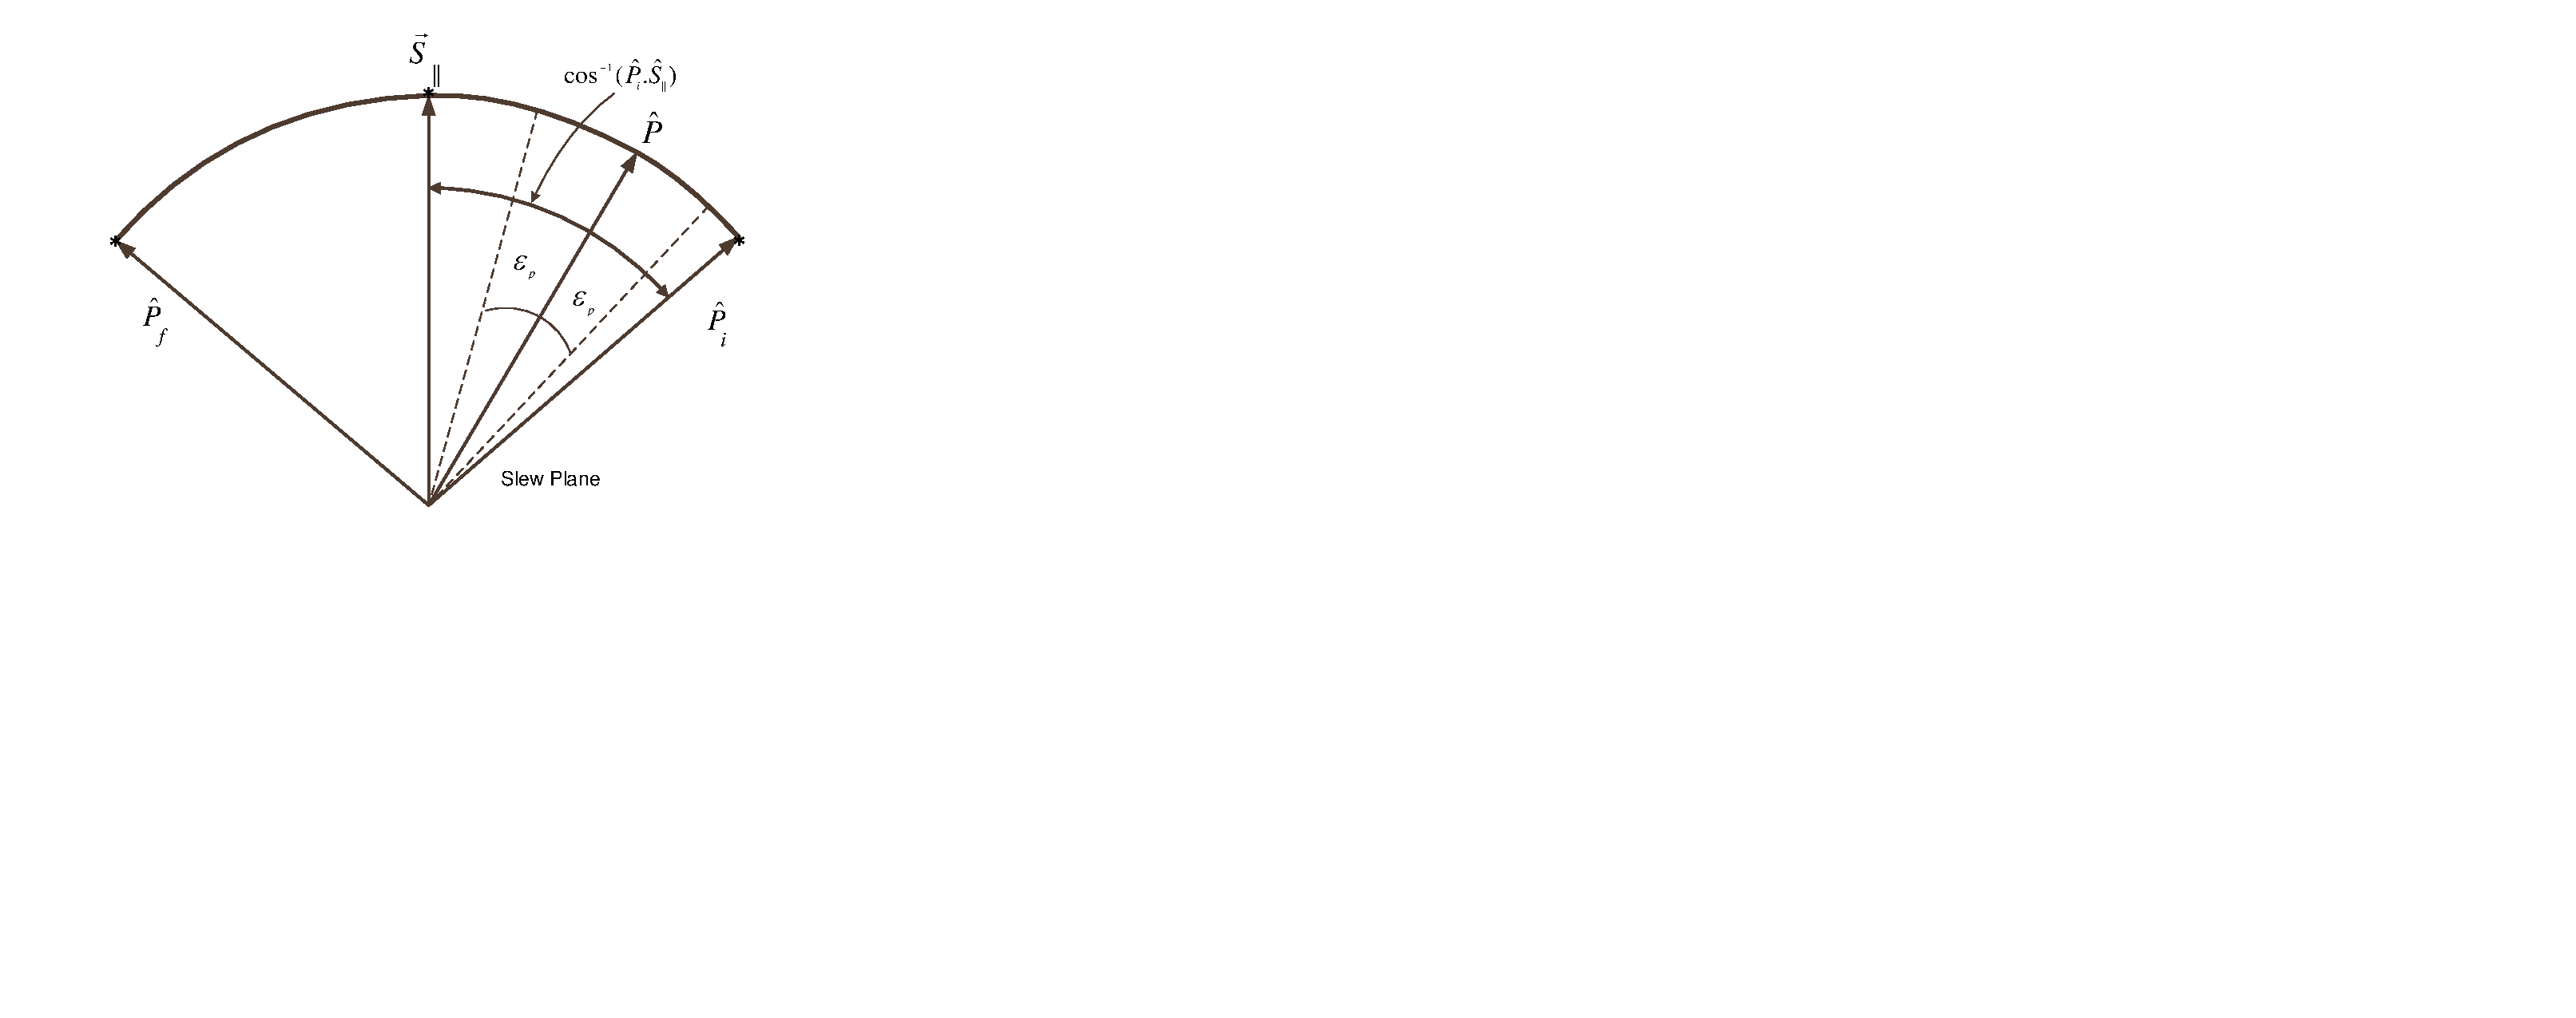
\includegraphics[width=1.75in]{./Figures/SVAS_1r_modified}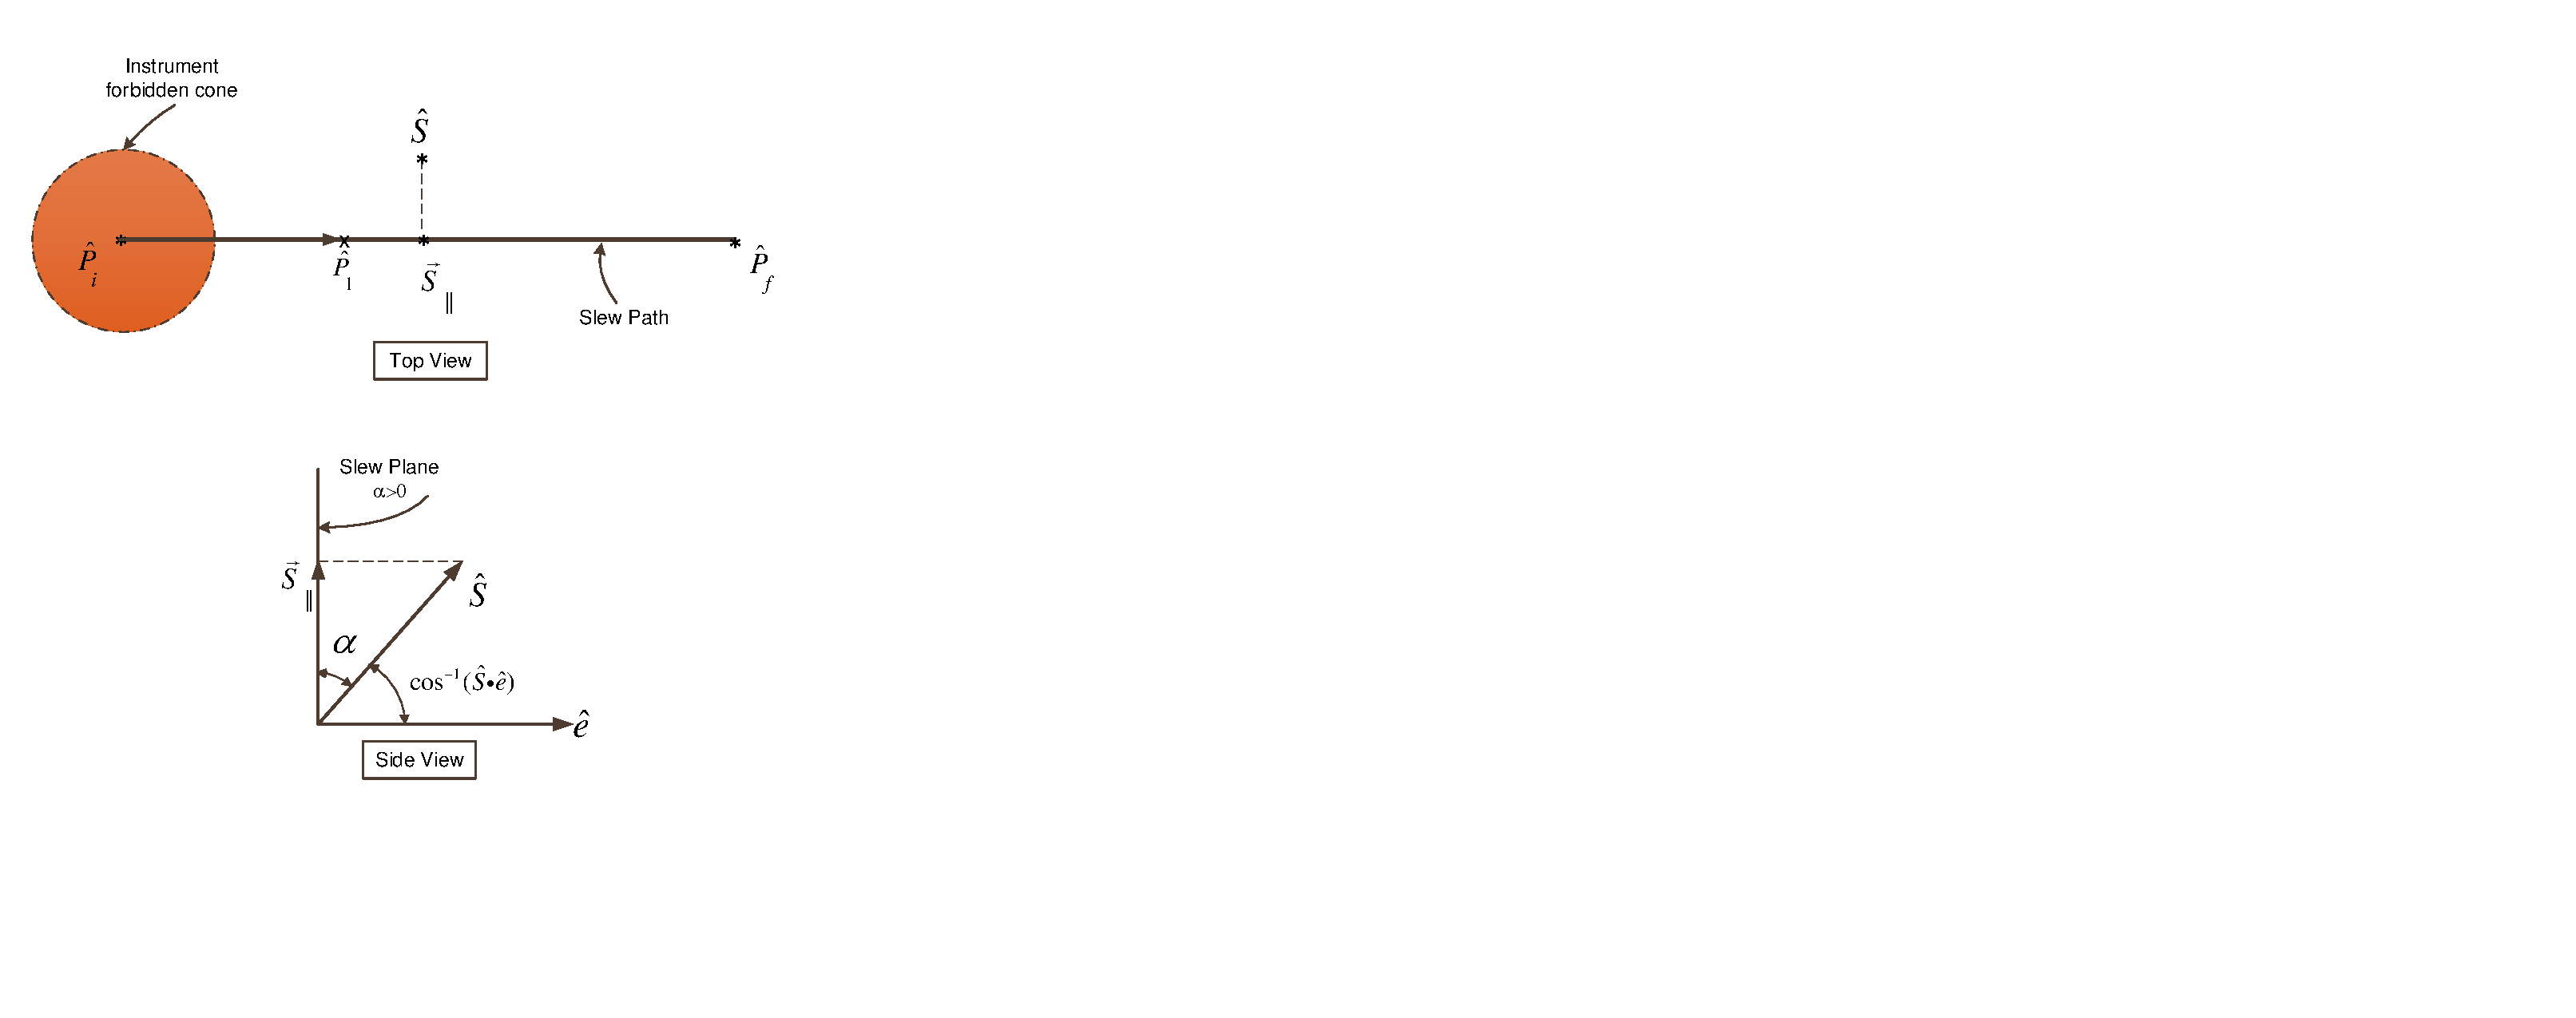
\includegraphics[width=2in]{./Figures/SVAS_1rb_modified}
\end{figure}
\end{block}
\end{frame}
%
%%-------------------------------------------------------------------------------------------------------------------------------------------------------------------
\begin{frame}{Sun-Avoidance Slew (SAS) Algorithm}
\begin{block}{Slew Maneuvers}
\begin{enumerate}[2]
\item The $2^{nd}$ slew around the unit sun vector, $\hat{S}$, via $\phi_2$.
\begin{enumerate}[a]
\item when $\alpha\neq0$
\end{enumerate}
\end{enumerate}
\begin{equation}
\phi_2=2\tan^{-1}\Big[ \frac{\hat{S}\cdot (\hat{P}_1\times\hat{S}_{||})}{(\hat{P}_1\cdot\hat{S}_{||})-(\hat{S}\cdot\hat{P}_1)(\hat{S}\cdot\hat{S}_{||})}\Big],
\end{equation}
\begin{figure}
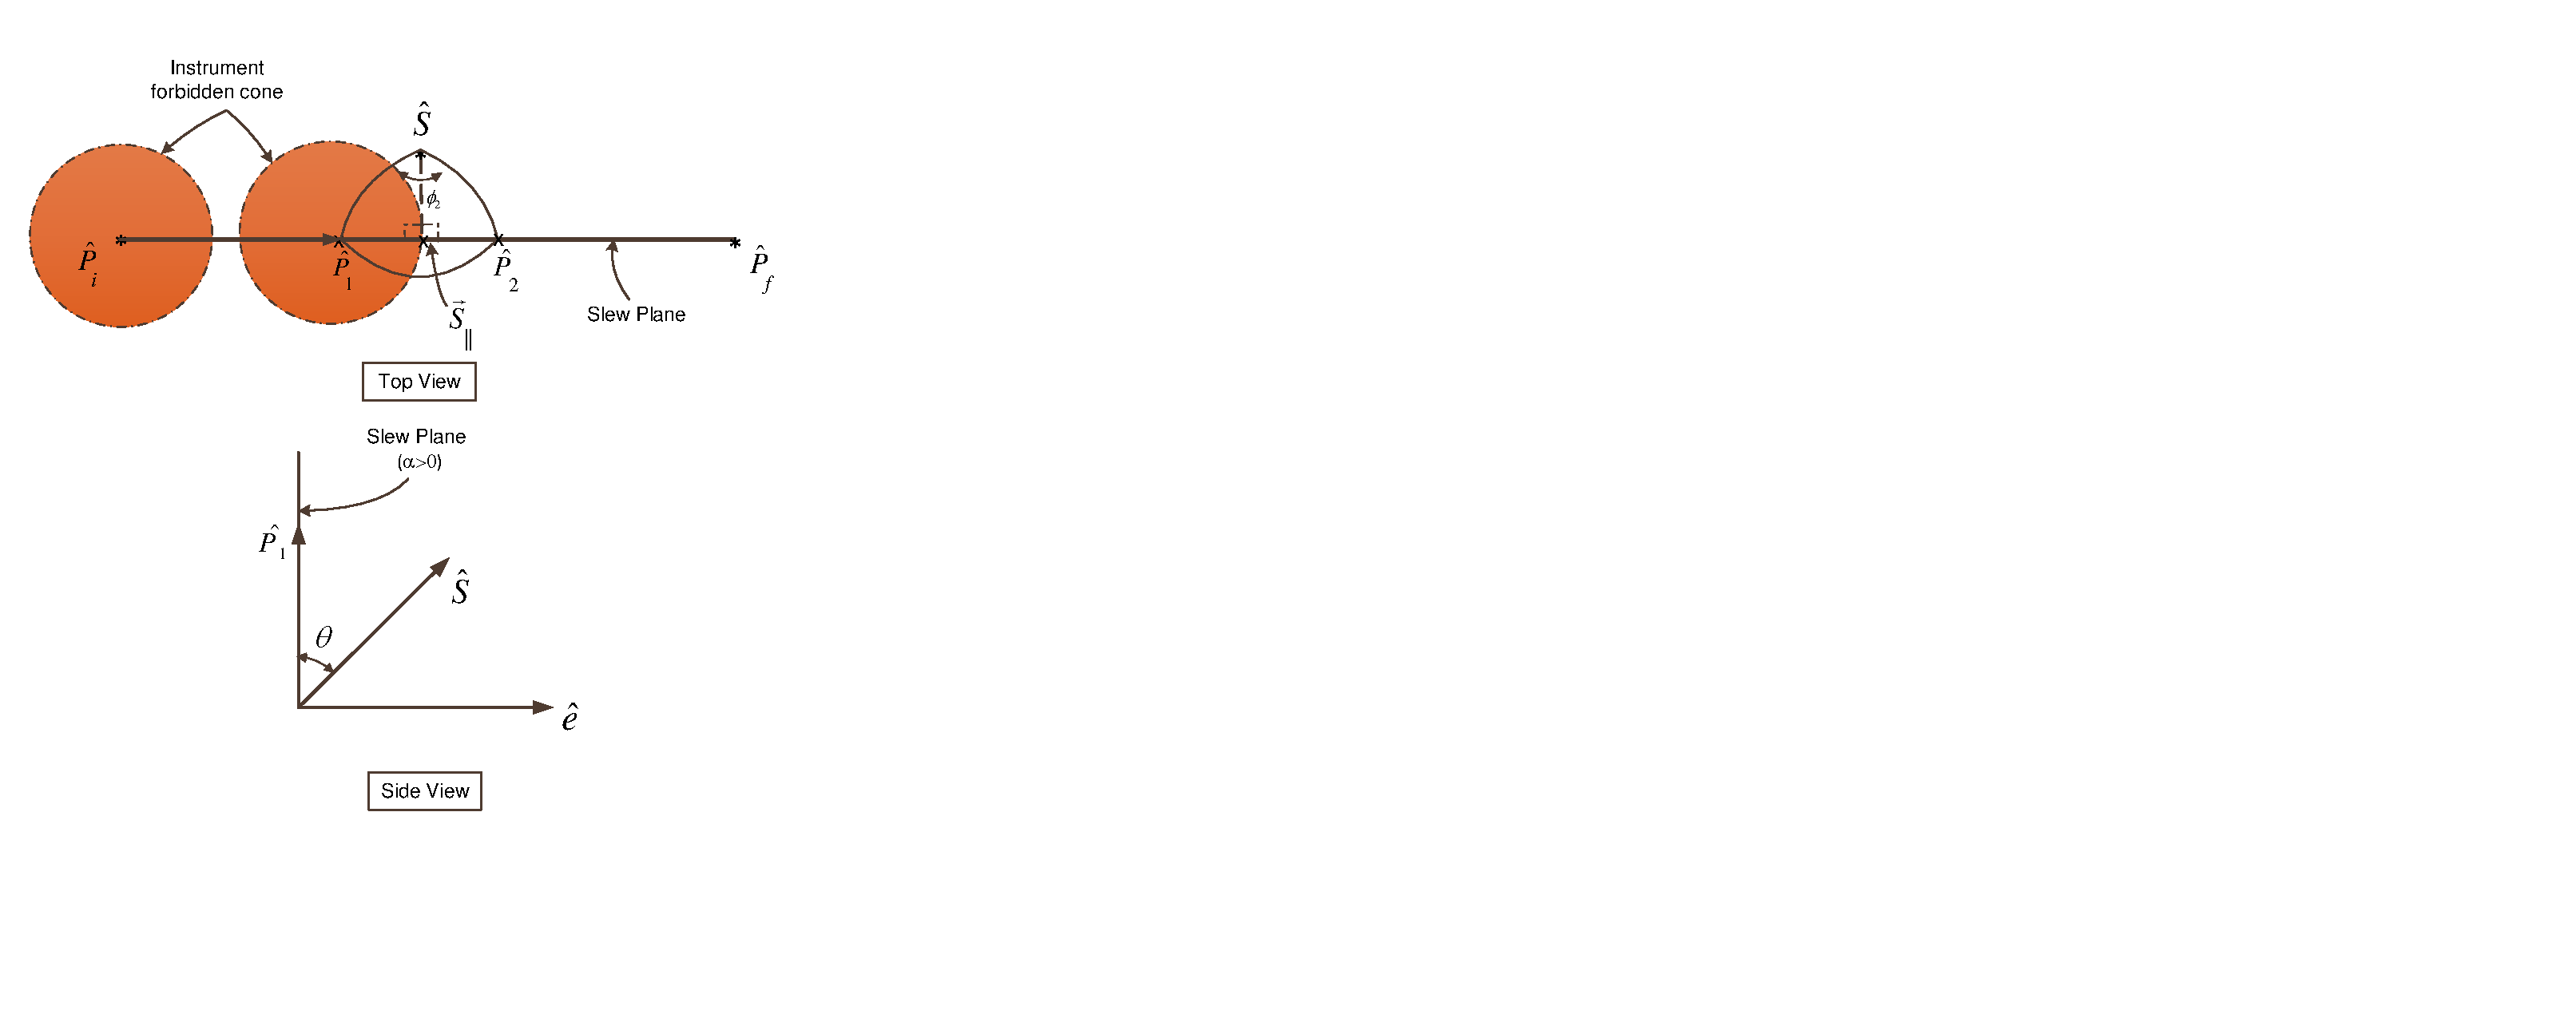
\includegraphics[width=2in]{./Figures/SVAS_2r_modified}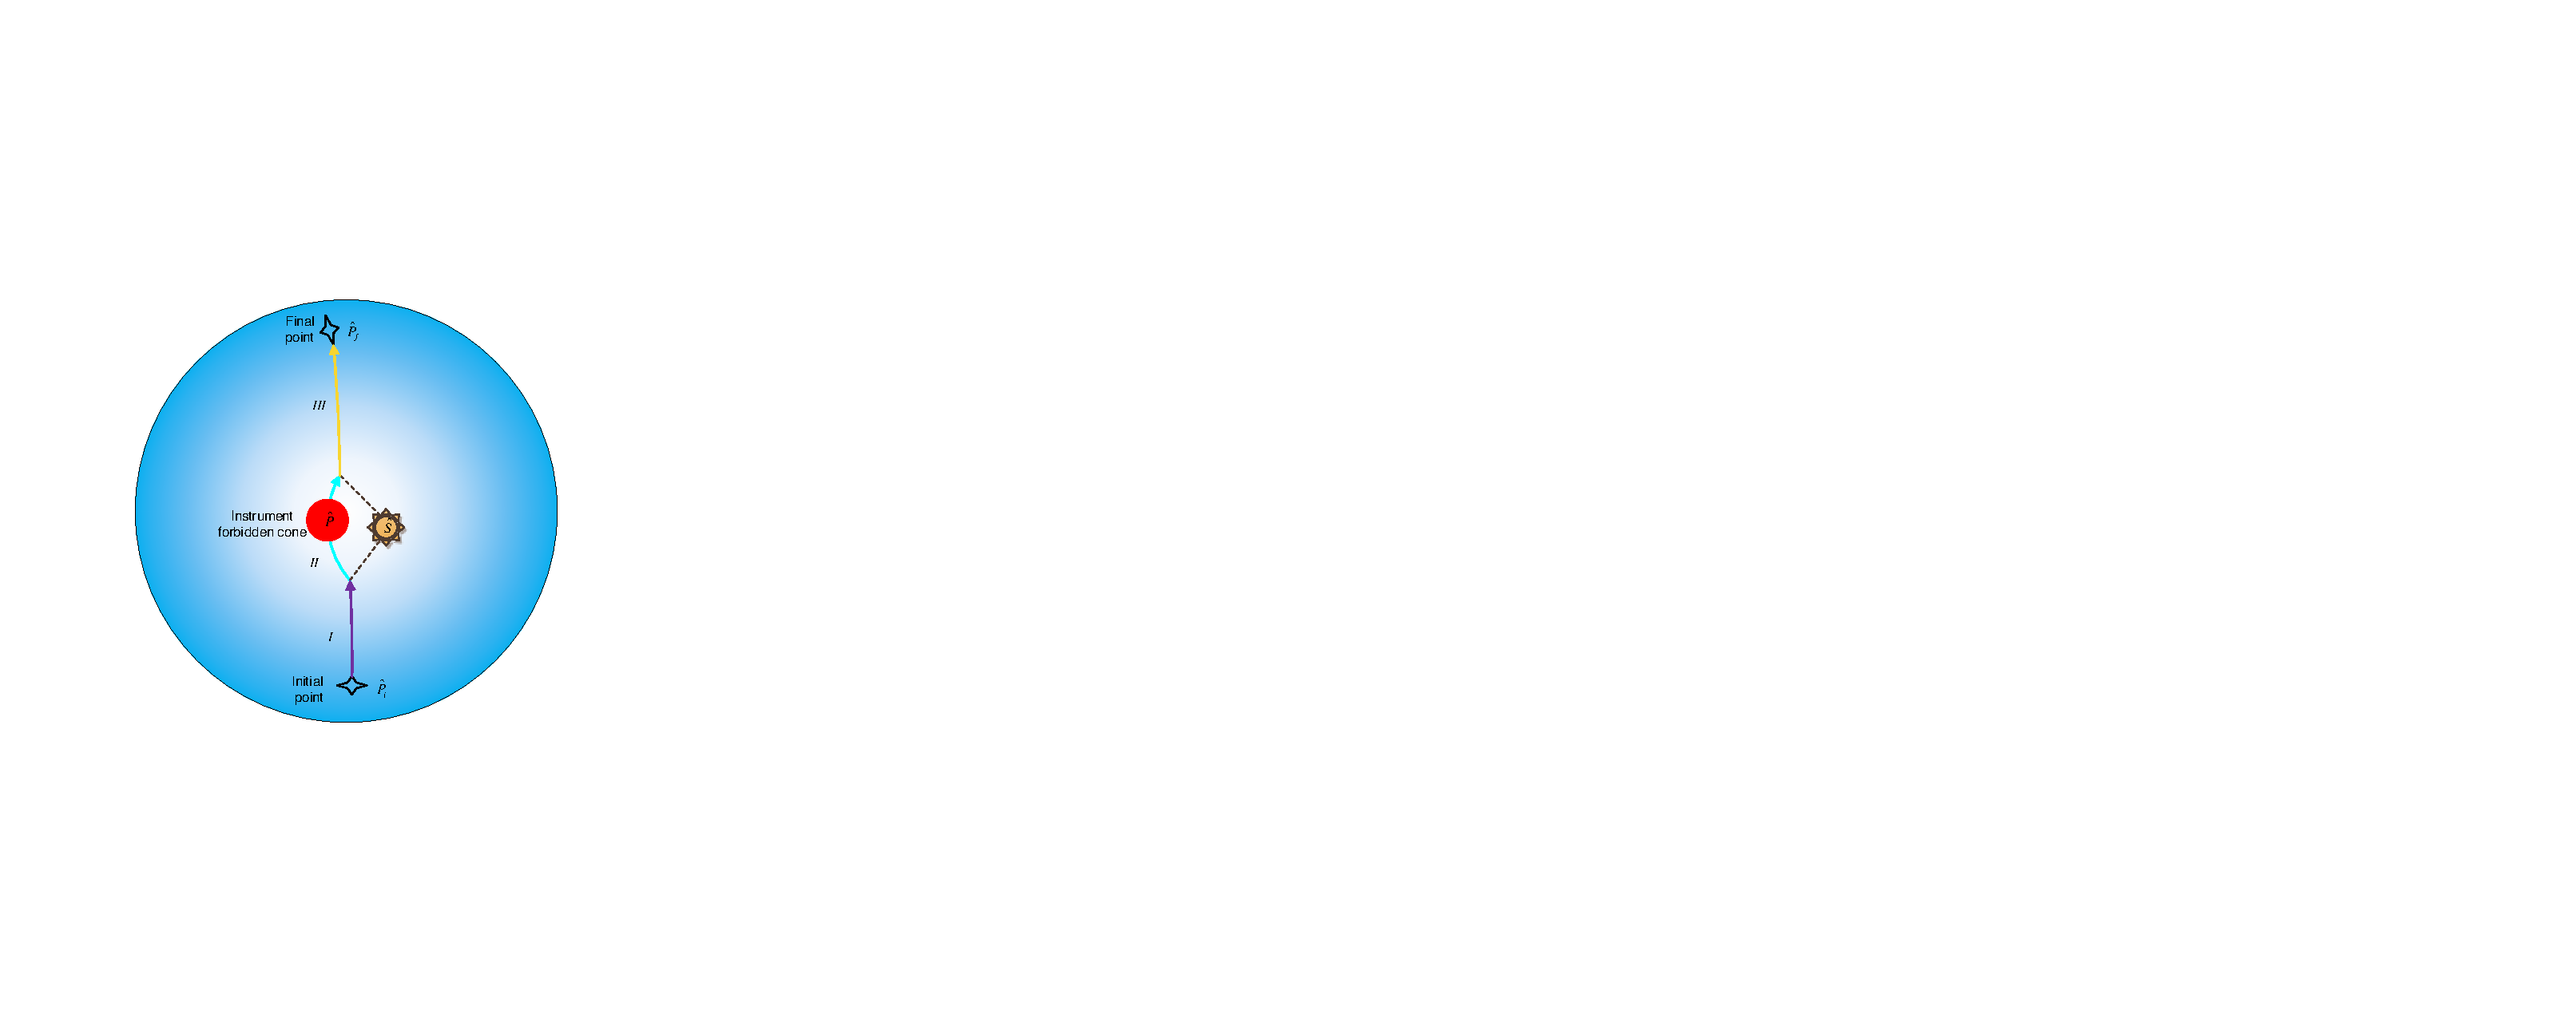
\includegraphics[width=1.5in]{./Figures/SASSchematic4}
\end{figure}


%		\begin{figure}
%			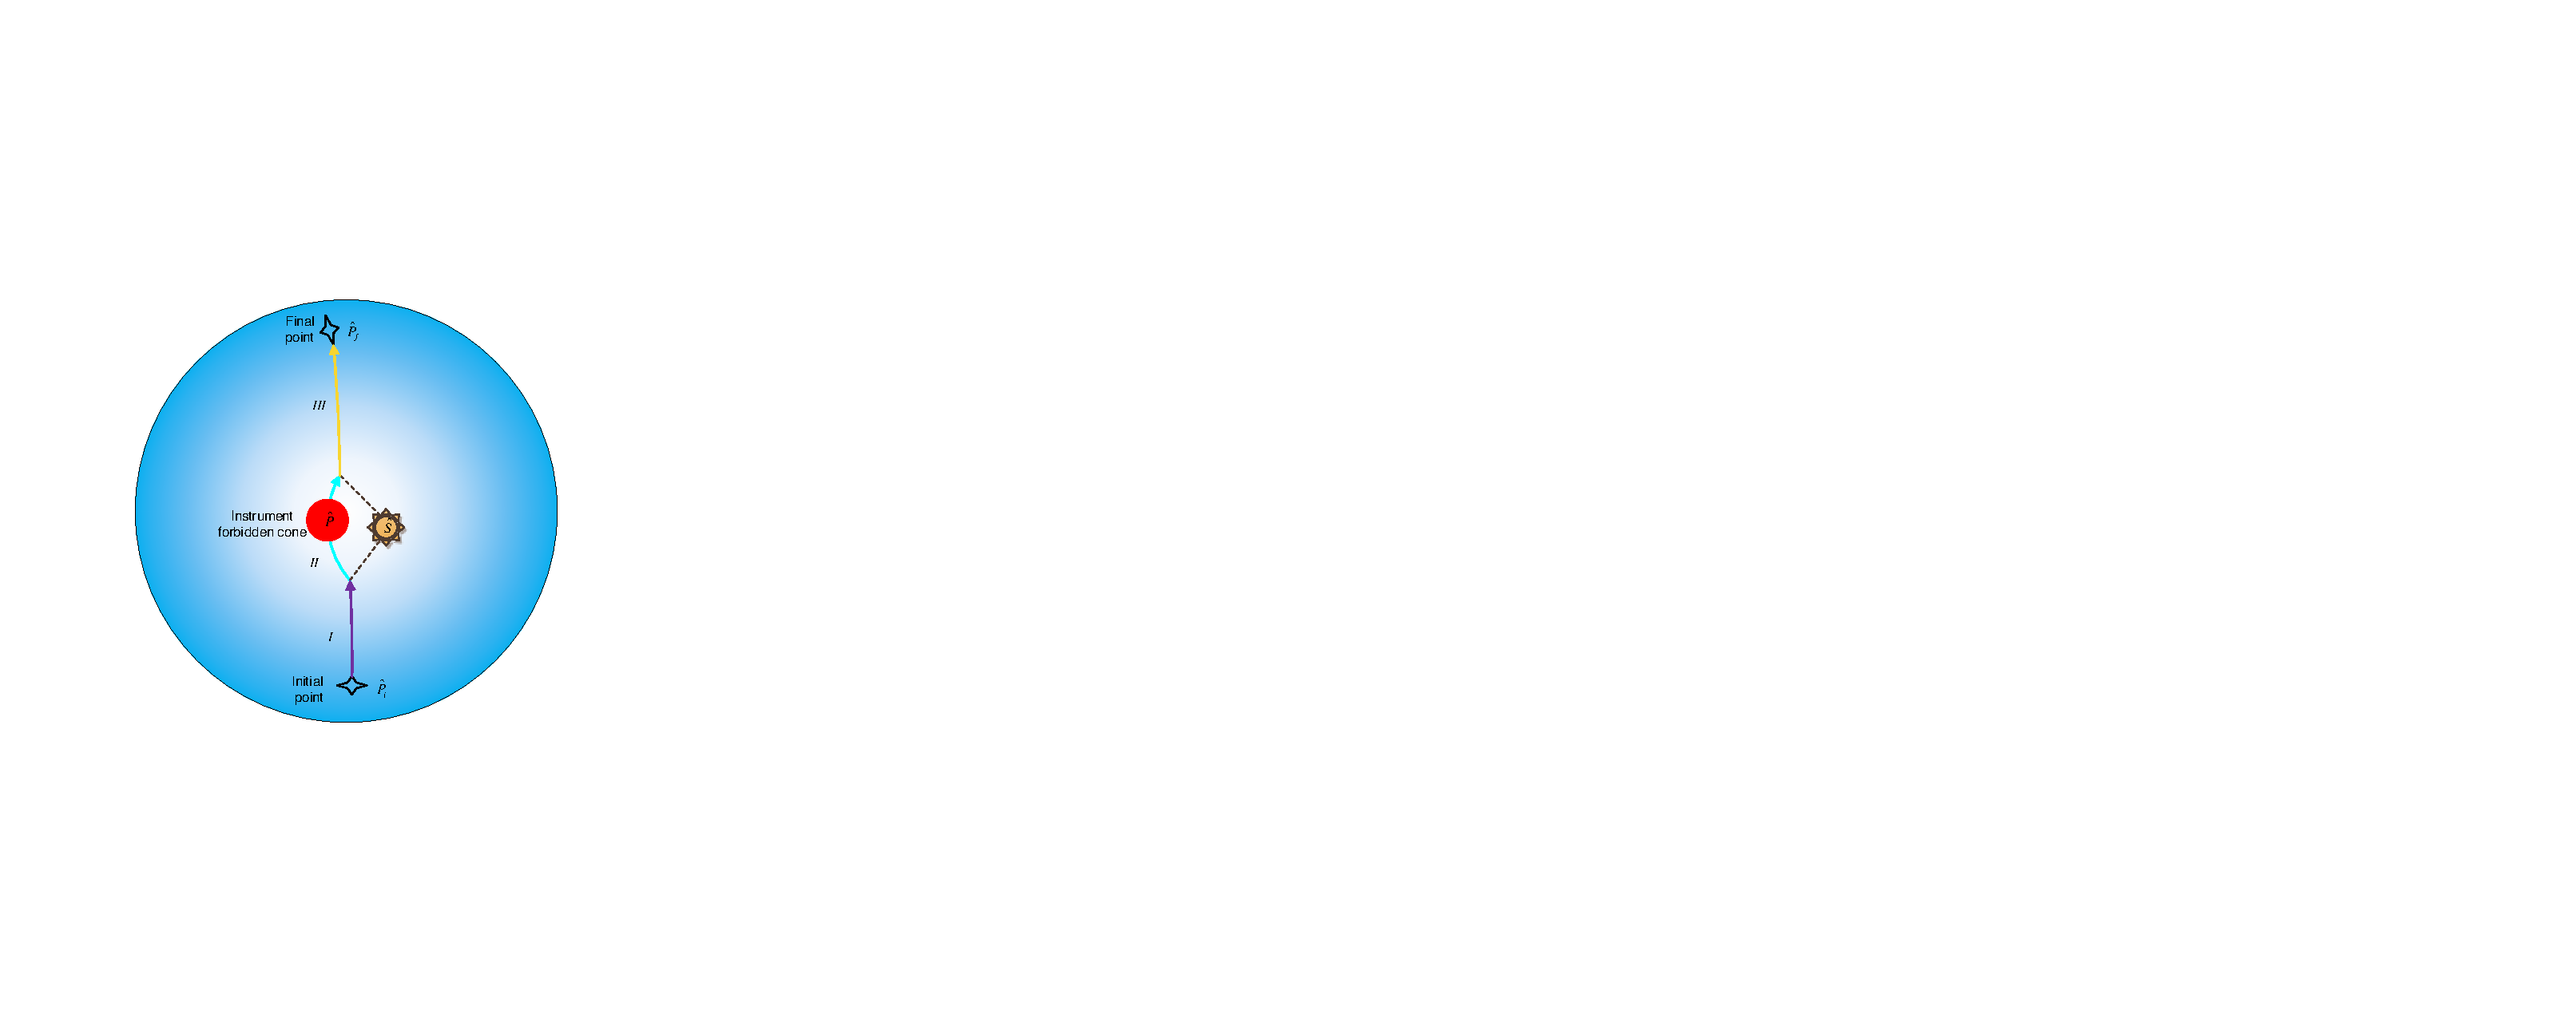
\includegraphics[width=1.5in]{./Figures/SASSchematic4}
%		\end{figure}

\end{block}
\end{frame}
%%-------------------------------------------------------------------------------------------------------------------------------------------------------------------
\begin{frame}{Sun-Avoidance Slew (SAS) Algorithm}
\begin{block}{Slew Maneuvers}
\begin{enumerate}[2]
\item The $2^{nd}$ slew around the unit sun vector, $\hat{S}$, via $\phi_2=180^{\circ}$.
\begin{enumerate}[b)]
\item when $\alpha=0$
\end{enumerate}
\end{enumerate}
\begin{figure}
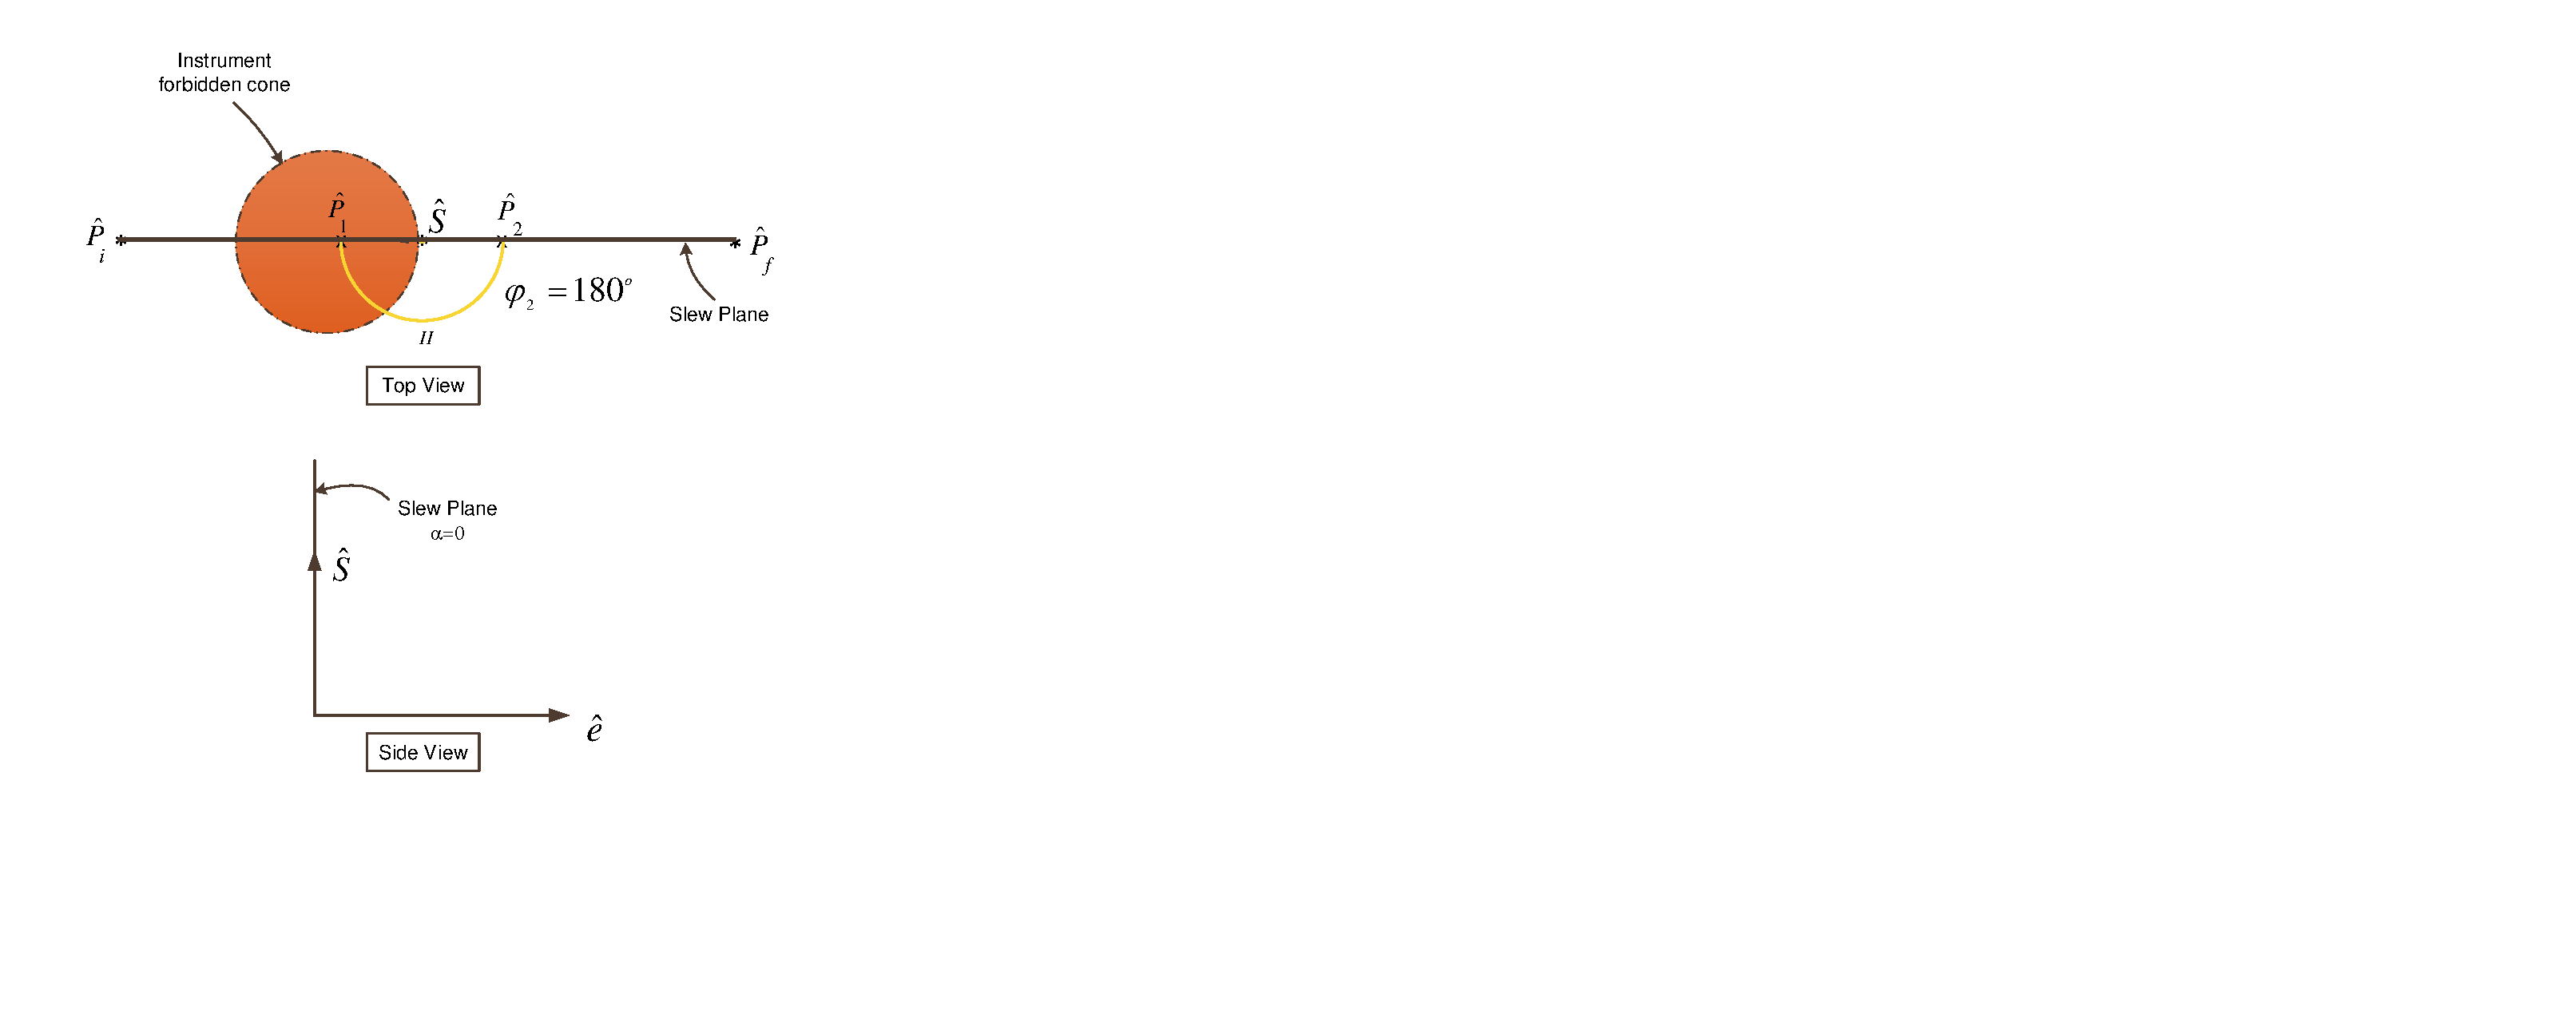
\includegraphics[width=2in]{./Figures/SVAS_3r_modified}
\end{figure}
\end{block}
\end{frame}

%%-------------------------------------------------------------------------------------------------------------------------------------------------------------------
\begin{frame}{Sun-Avoidance Slew (SAS) Algorithm}
\begin{block}{Slew Maneuvers}
\begin{enumerate}[3]
\item The $3^{rd}$ slew about the $\hat{e}$ through angle:
 \begin{equation}
 \phi_3=\left\{
                \begin{array}{ll}
                  \cos^{-1}(_G\hat{P}_f.\hat{P}_2)& when\  _G\hat{P}_f.\hat{P}_2\geq 0\\
                 \cos^{-1}(_G\hat{P}_f.\hat{P}_2)-2\pi& when\ _G\hat{P}_f.\hat{P}_2<0\\
                \end{array}
              \right.
 \end{equation}
\begin{figure}
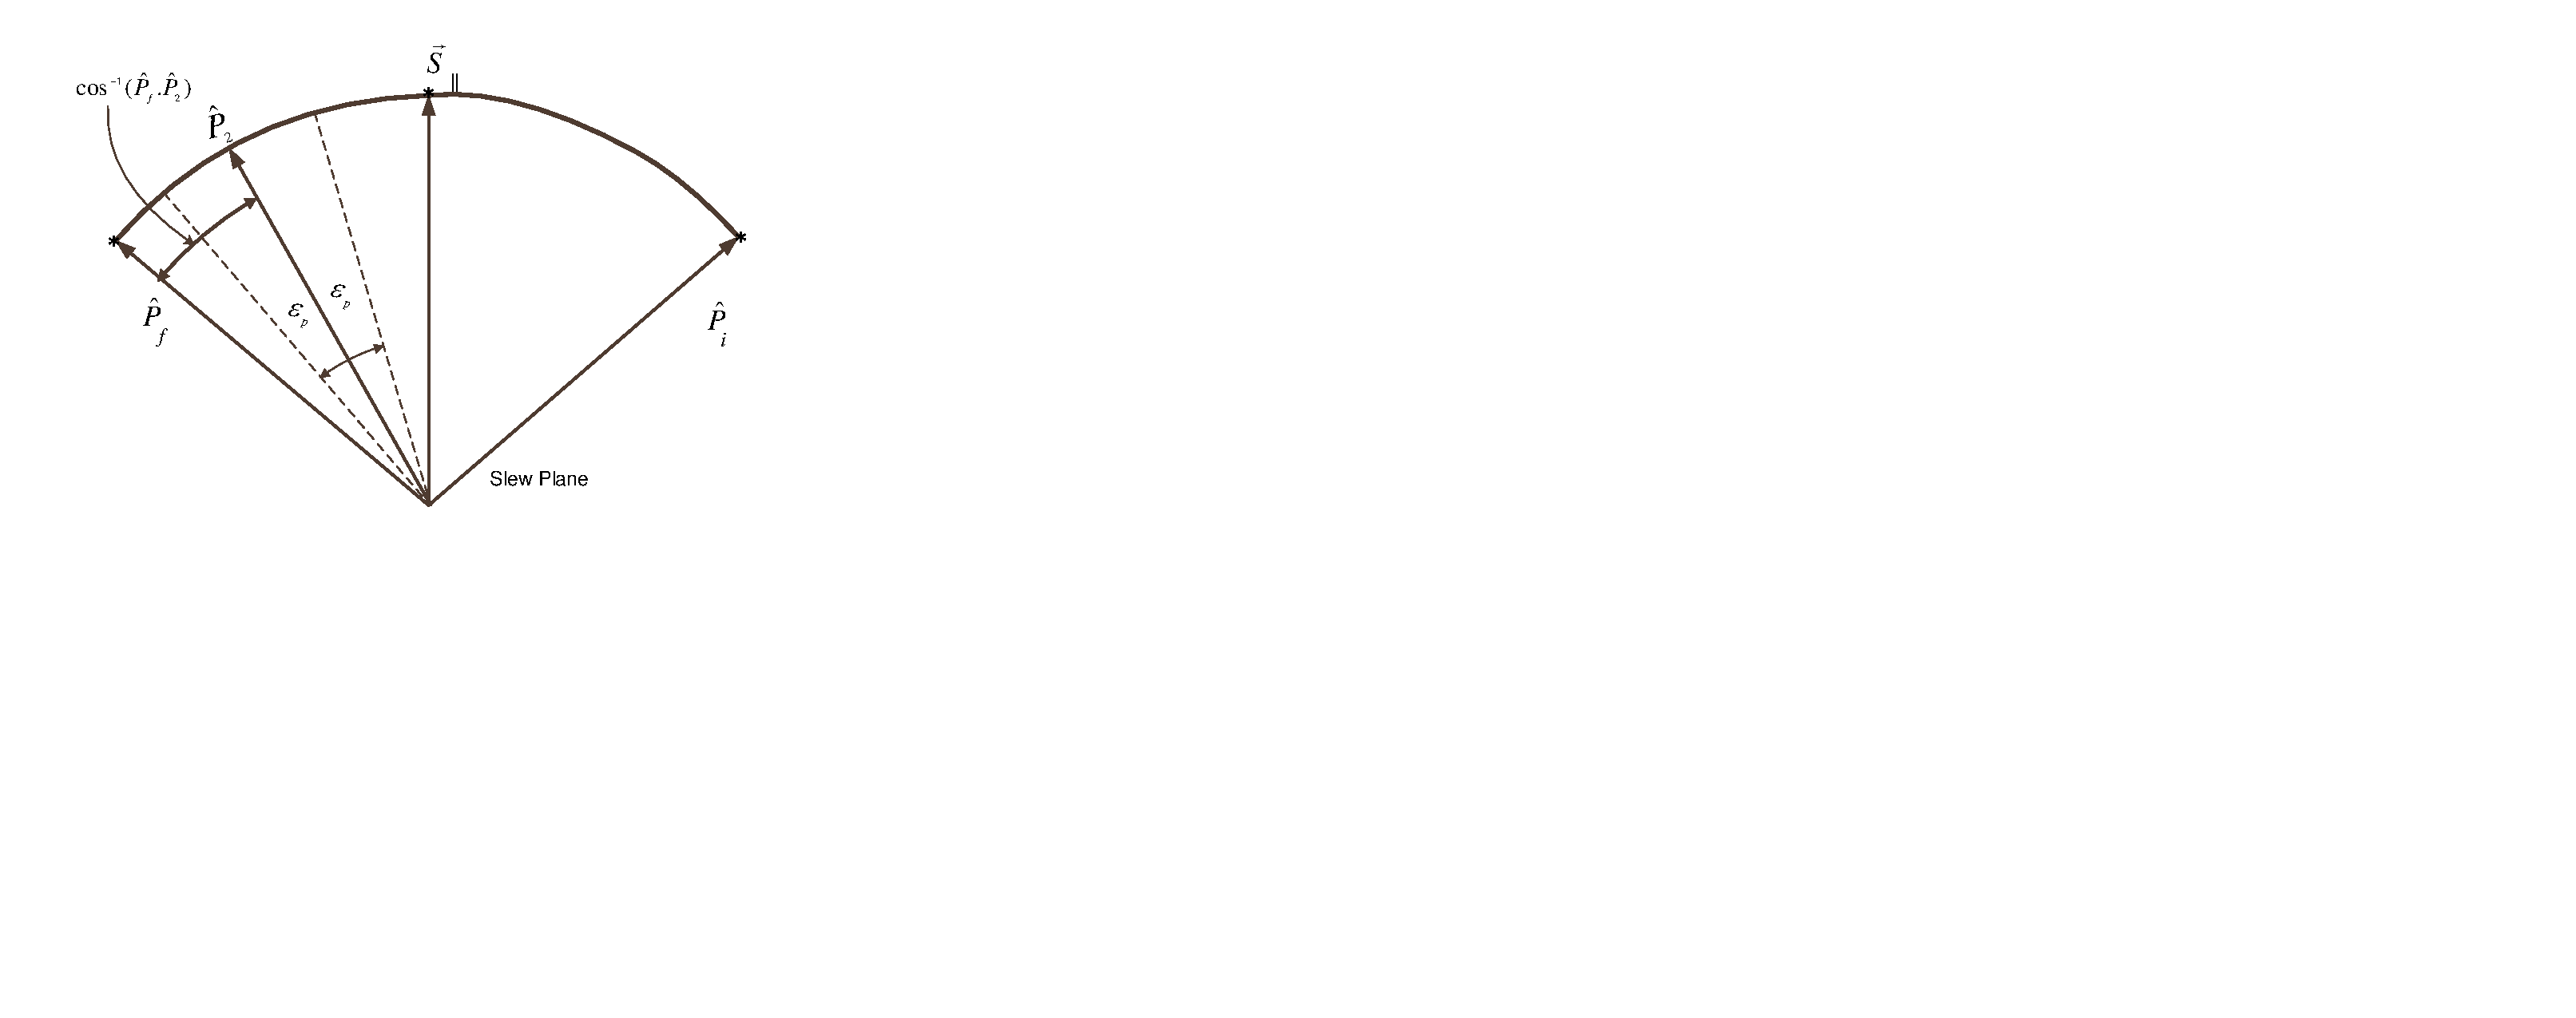
\includegraphics[width=2in]{./Figures/SVAS_4r}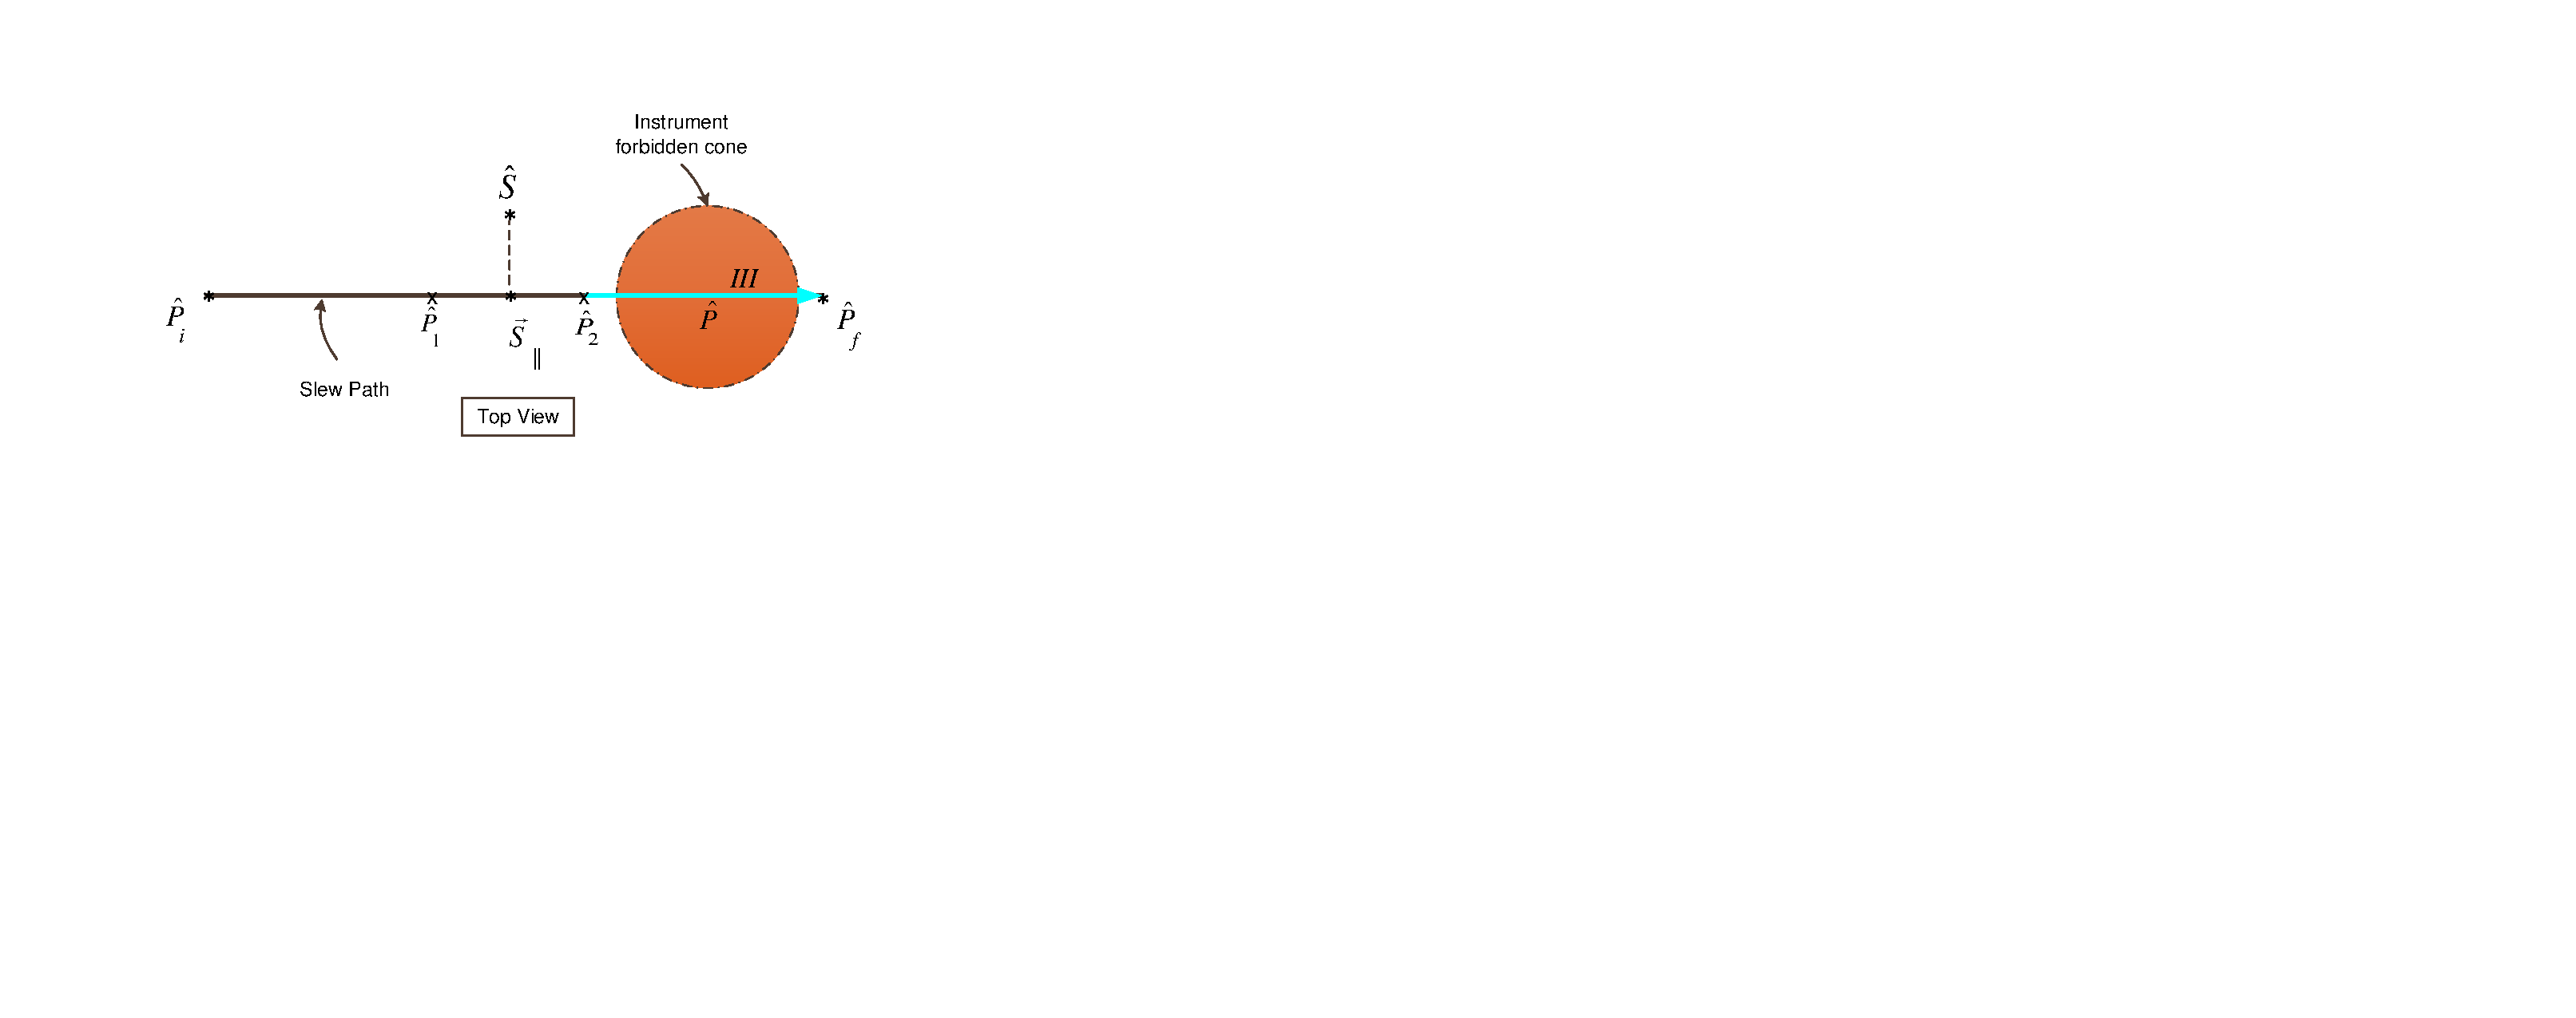
\includegraphics[width=2in]{./Figures/SVAS_4r_modified.pdf}
\end{figure}
\end{enumerate}
\begin{enumerate}[4]
\item The final slew is about the instrument boresight axis to go to the final attitude. 
\end{enumerate}
\end{block}
\end{frame}
%
%
%%-------------------------------------------------------------------------------------------------------------------------------------------------------------------
\begin{frame}{Summary of the Algorithm}
\begin{block}{}
\begin{enumerate}
\item Slew around the eigenaxis,$\hat{e}$, through angle:

 \begin{equation}\label{phi1}
 \phi_1=\left\{
                \begin{array}{ll}
                 \cos^{-1}(\hat{P}_i\cdot_\mathcal{G}\hat{S}_{||})-\epsilon_p& when\  \cos^{-1}(\hat{P}_i\cdot_\mathcal{G}\hat{S}_{||})-\epsilon_p\leq \pi\\
                 \cos^{-1}(\hat{P}_i\cdot_\mathcal{G}\hat{S}_{||})-\epsilon_p-2\pi& when\ \cos^{-1}(\hat{P}_i\cdot_\mathcal{G}\hat{S}_{||})-\epsilon_p>\pi\\
                \end{array}
              \right.
 \end{equation}
\item Slew around the $\hat{S}$ via:

 \begin{equation}\label{phi2}
 \phi_2=\left\{
                \begin{array}{ll}
                \phi_2=2\tan^{-1}\Big[ \frac{\hat{S}\cdot (\hat{P}_1\times\hat{S}_{||})}{(\hat{P}_1\cdot\hat{S}_{||})-(\hat{S}\cdot\hat{P}_1)(\hat{S}\cdot\hat{S}_{||})}\Big],& when\  \alpha\neq 0\\
                 \pi& when\ \alpha=0\\
                \end{array}
              \right.
 \end{equation}
 \item Slew about the $\hat{e}$ through angle:
 \begin{equation}\label{phi3}
 \phi_3=\left\{
                \begin{array}{ll}
                  \cos^{-1}(_\mathcal{G}\hat{P}_f.\hat{P}_2)& when\  _\mathcal{G}\hat{P}_f.\hat{P}_2\geq 0\\
                 \cos^{-1}(_\mathcal{G}\hat{P}_f.\hat{P}_2)-2\pi& when\ _\mathcal{G}\hat{P}_f.\hat{P}_2<0\\
                \end{array}
              \right.
 \end{equation}

\item Perform the final rotation, $\phi_4$, about the instrument boresight axis to adjust the attitude. 
\end{enumerate}
\end{block}
\end{frame}
%
%
%
%
%%-------------------------------------------------------------------------------------------------------------------------------------------------------------------
\begin{frame}
\begin{block}{}
\begin{center}
{\LARGE{Computing the Steering Profiles}}
\begin{center}
 Single-Axis, Agile Slew Maneuver with Velocity and Acceleration Constraints.
\end{center}
\end{center}
\end{block}
\end{frame}
%%-------------------------------------------------------------------------------------------------------------------------------------------------------------------
\section{Computing Steering Profiles}
\begin{frame}{Computing Steering Profiles}
\begin{block}{ Problem Statement}
Consider the motion of a \textcolor{blue}{rigid} spacecraft around a given inertially-fixed axis, $_G\hat{e}=[e_x,e_y,e_z]^T$. The problem of minimum-time slew maneuver around the $\hat{e}$ axis can be formulated as

%\begin{columns}
\begin{minipage}{0.55\textwidth}
\begin{equation}\label{costfunction}
\underset{u}{Minimze}\ J[x(.), u(.), t_f]=\int_{t0}^{t_f} dt,
\end{equation}
subject to the following dynamic constraint
\begin{equation}\label{system}
 \Sigma:\left\{
                \begin{array}{l}
                \dot{x}_1=x_2, \\
                \dot{x}_2=M/I_{\hat{e}}^{G/G*}=u, \\
                \end{array}
              \right.
 \end{equation}
where $x_1\triangleq\phi$ and $x_2=\dot{\phi}$. 
\end{minipage}
\begin{minipage}{0.35\textwidth}
\begin{center}
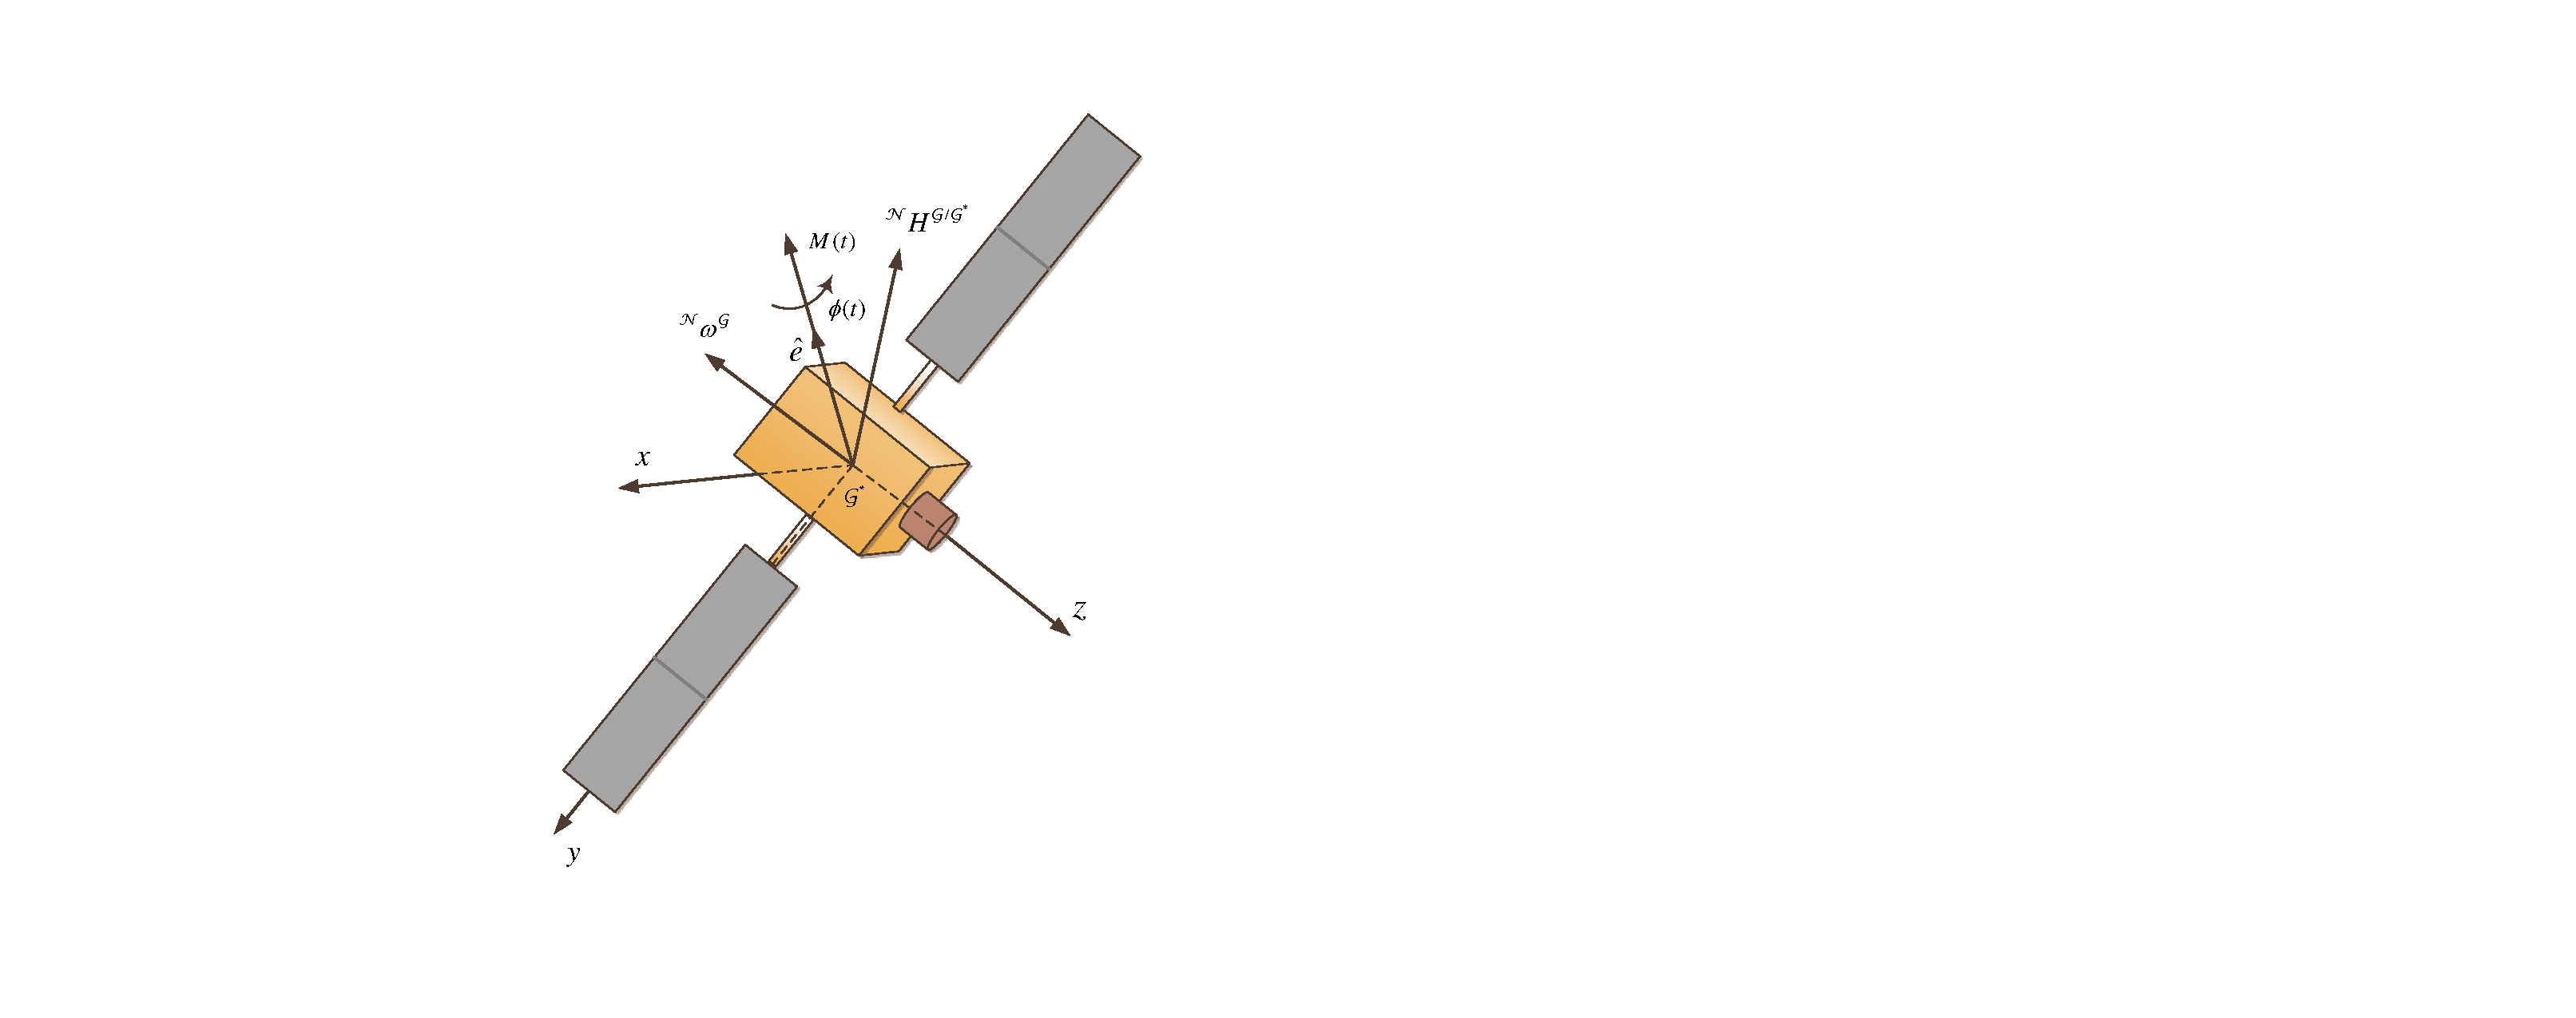
\includegraphics[width=2.25in]{./Figures/Spacecraft}      
\end{center}
\end{minipage}
%\end{columns}
\end{block}
\end{frame}
%%-------------------------------------------------------------------------------------------------------------------------------------------------------------------
\begin{frame}{Computing Steering Profiles}
\begin{block}{ Problem Statement Continued}
The boundary conditions are
\begin{equation}\label{Bcs}
 BCs:\left\{
                \begin{array}{l}
                \phi(t_0)=0, \phi(t_f)=\phi_{f},\\
               \dot{\phi}(t_0)=\dot{\phi}_{0},\dot{ \phi}(t_f)=\dot{\phi}_{f}, \\
                \end{array}
              \right.
 \end{equation}
and velocity (state) and acceleration (control) constraints are

\begin{equation}\label{constraints1}
 C_1:\left\{
                \begin{array}{l}
               |x_2=\dot{\phi}|\leq \dot{\phi}_{max},\\
              |u=\ddot{\phi}|\leq \ddot{\phi}_{max},\\
                \end{array}
              \right.
 \end{equation}
%in which
%\begin{equation}
%\dot{\phi}_{max}=[I^{w/w^*}]^{-1}[^NH^{G/G*}-(I^{G/G*}+I^{w/w*})^N\omega^G]/(e_x+e_y+e_z),
%\end{equation}
%
%
%%\end{minipage}
%%\begin{minipage}{0.35\textwidth}
%%\begin{center}
%%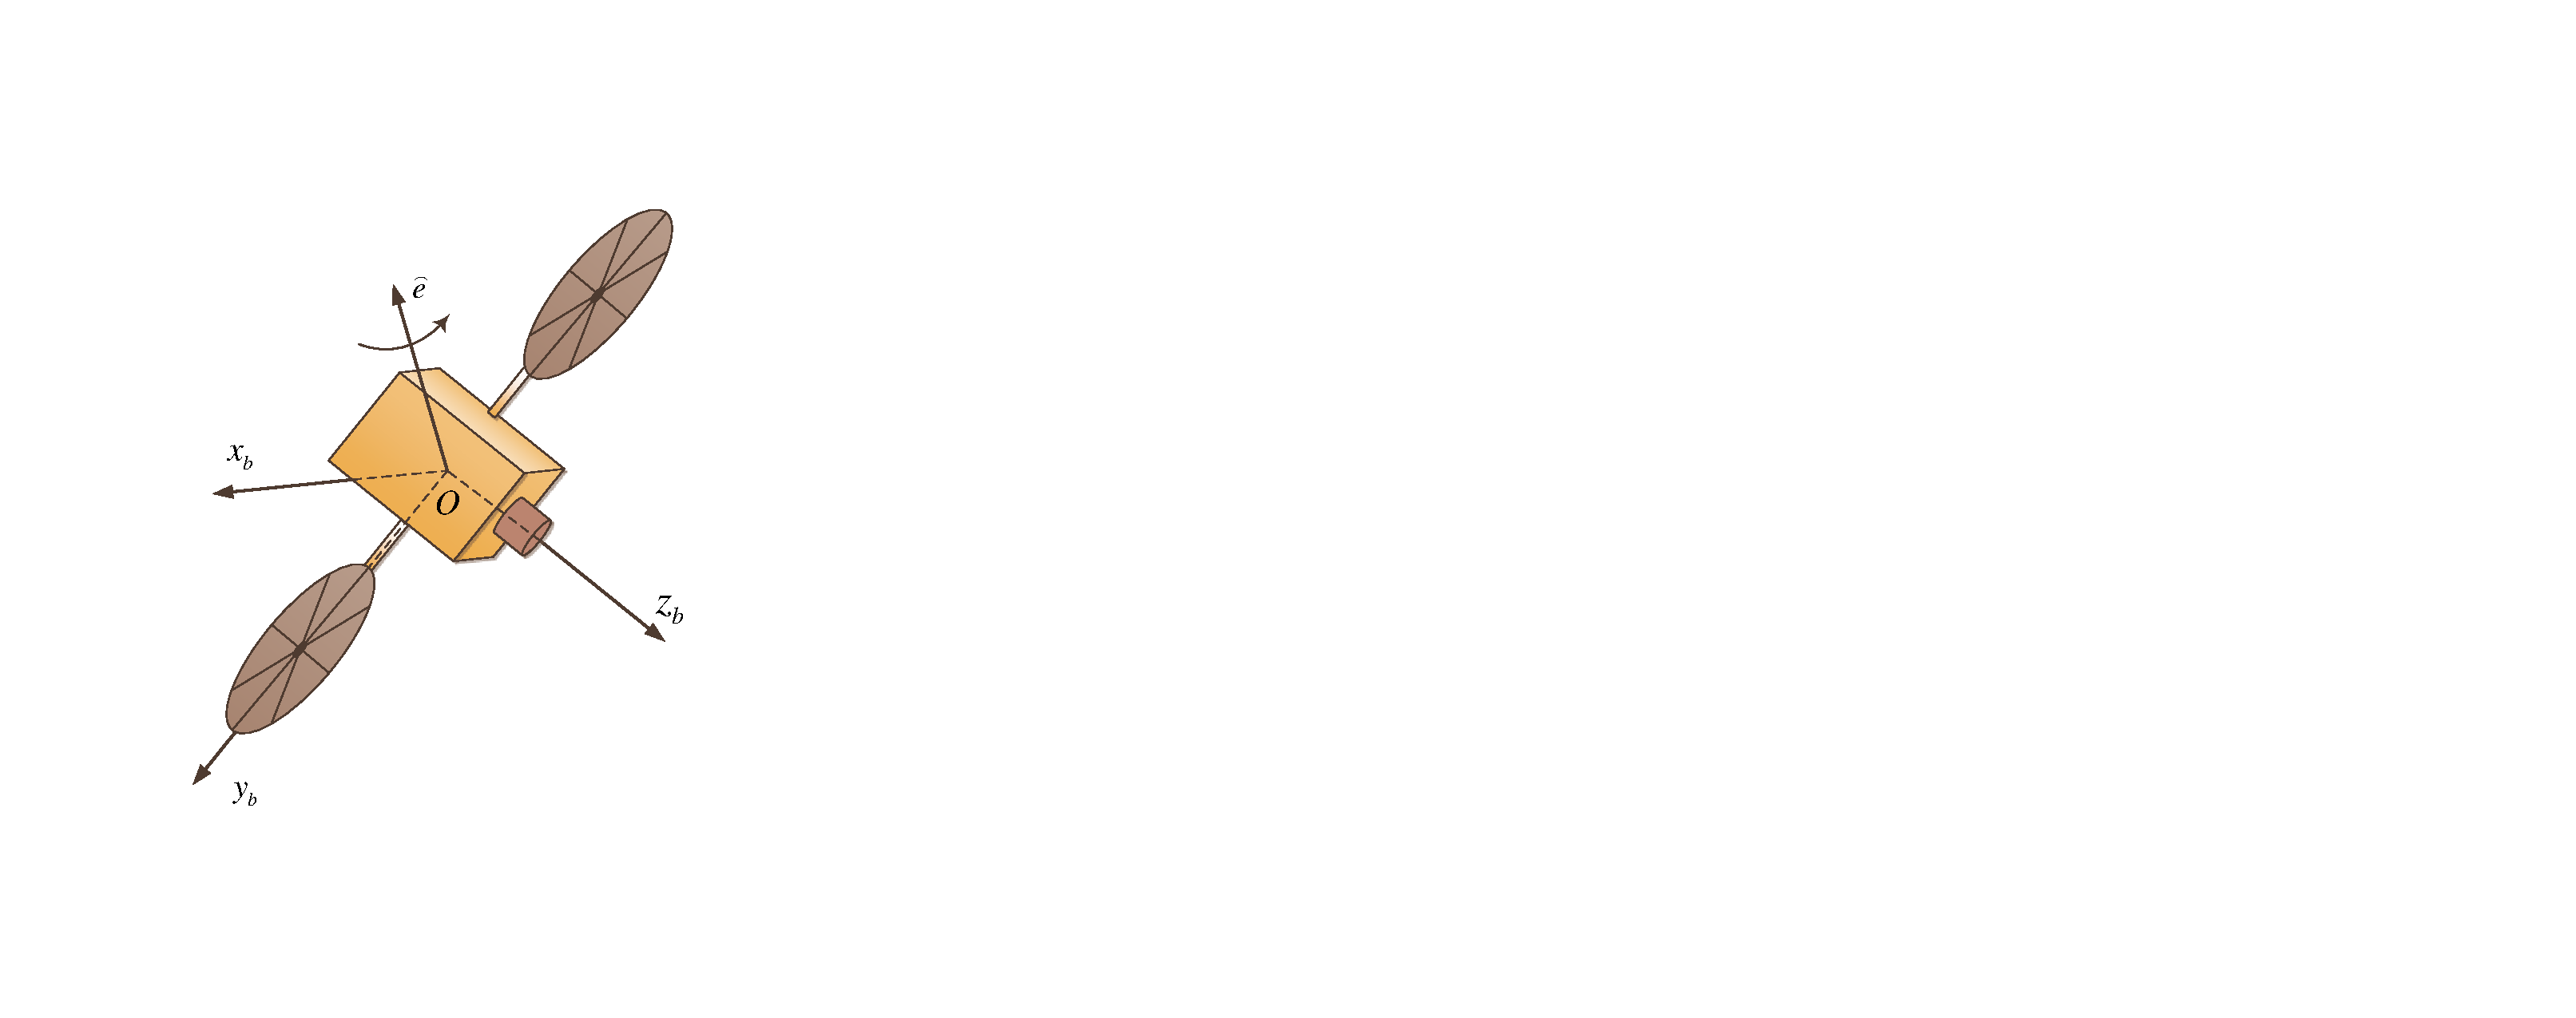
\includegraphics[width=2in]{./Spacecraft3}      
%%\end{center}
%%\end{minipage}
%%\end{columns}
%\end{block}
%\end{frame}
%%%-------------------------------------------------------------------------------------------------------------------------------------------------------------------
%\begin{frame}{Computing Steering Profiles}
%\begin{block}{ Problem Statement Continued}
% and
% \begin{equation}\label{phiddotmax}
%\ddot{\phi}_{max}=_B\hat{e}^T\  _BM_{max}/I_{\hat{e}}^{G/G*},
%\end{equation}
%where $^NH^{G/G*}$ is the total angular momentum of the gyrostat with respect to its center of mass, $G^*$, in the $N$-frame. $I^{G/G^*}$ and $I^{w/w*}$ represent the inertia dyadic of the gyrostat and reaction wheel with respect to their center of masses, respectively. $_BM_{max}$ is the maximum generated torque along the body-axes in the body frame.\\
%%Find the optimal steering laws: $^Bq^R$, $^B\omega^R$, and $^B\alpha^R$.
%\vspace{0.5in}

{\bf Find:} $\phi(t)$, $\dot{\phi}(t)$, and $\ddot{\phi}(t)$.
%\end{minipage}
%\begin{minipage}{0.35\textwidth}
%\begin{center}
%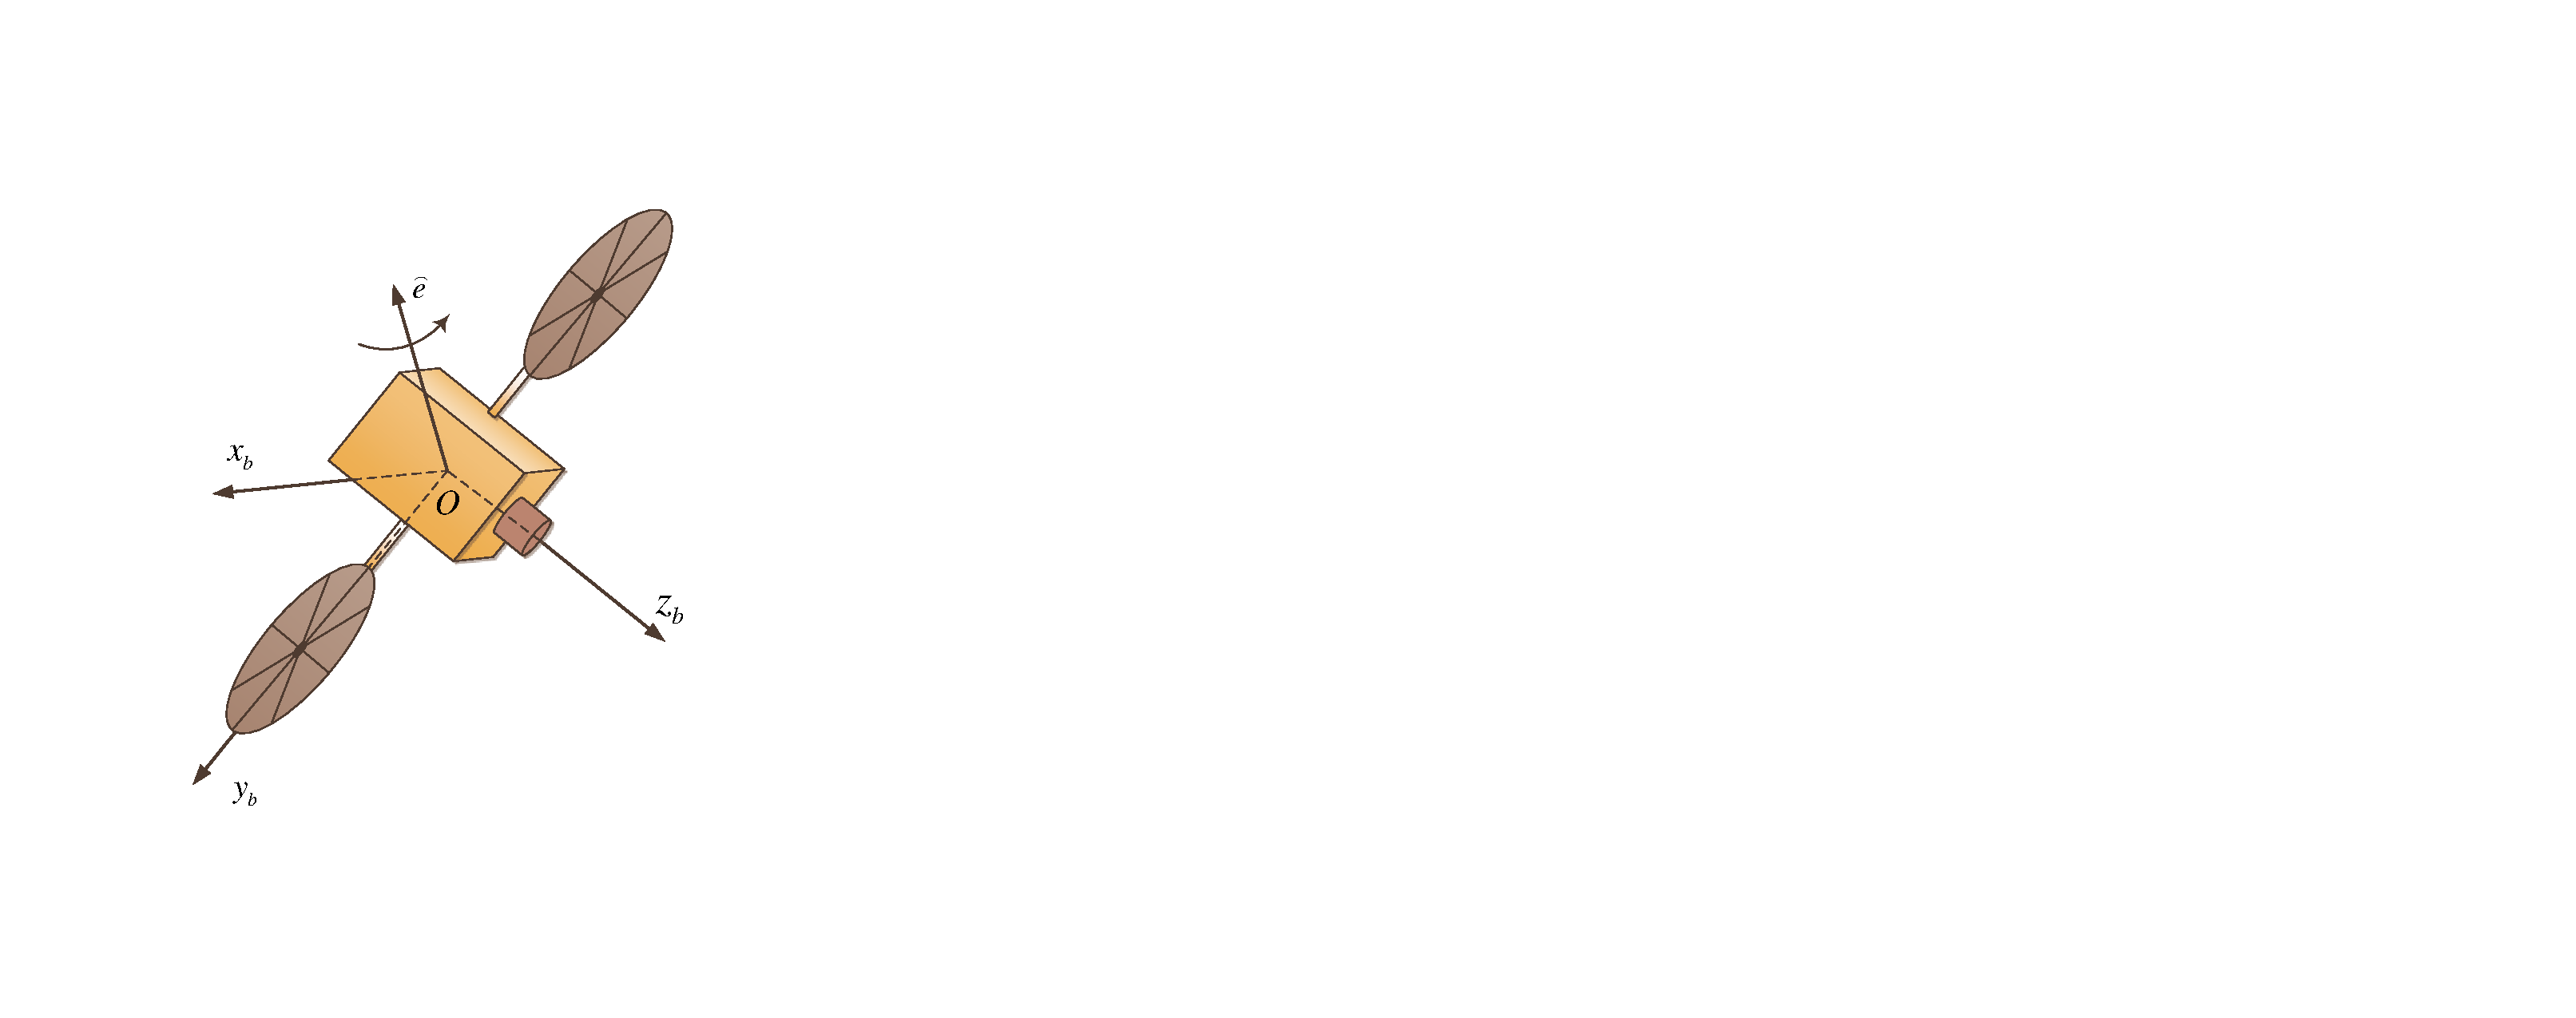
\includegraphics[width=2in]{./Spacecraft3}      
%\end{center}
%\end{minipage}
%\end{columns}
\end{block}
\end{frame}
%%-------------------------------------------------------------------------------------------------------------------------------------------------------------------
\begin{frame}{Computing Steering Profiles}

\begin{block}{ }
\small{
\begin{itemize}
\item Angular acceleration profile (bang-off-bang):
\end{itemize}
 \begin{equation}\label{phidd_cons}
 \ddot{\phi}(t)=u=\left\{
                \begin{array}{ll}
                \ddot{\phi}_{max}& when\  t_0\leq t\leq t_1,\\
                 0& when\  t_1\leq t \leq t_2,\\
                 -\ddot{\phi}_{max}& when \ t_2\leq t\leq t_f.
                \end{array}
              \right.
\begin{minipage}{0.35\textwidth}
\begin{center}
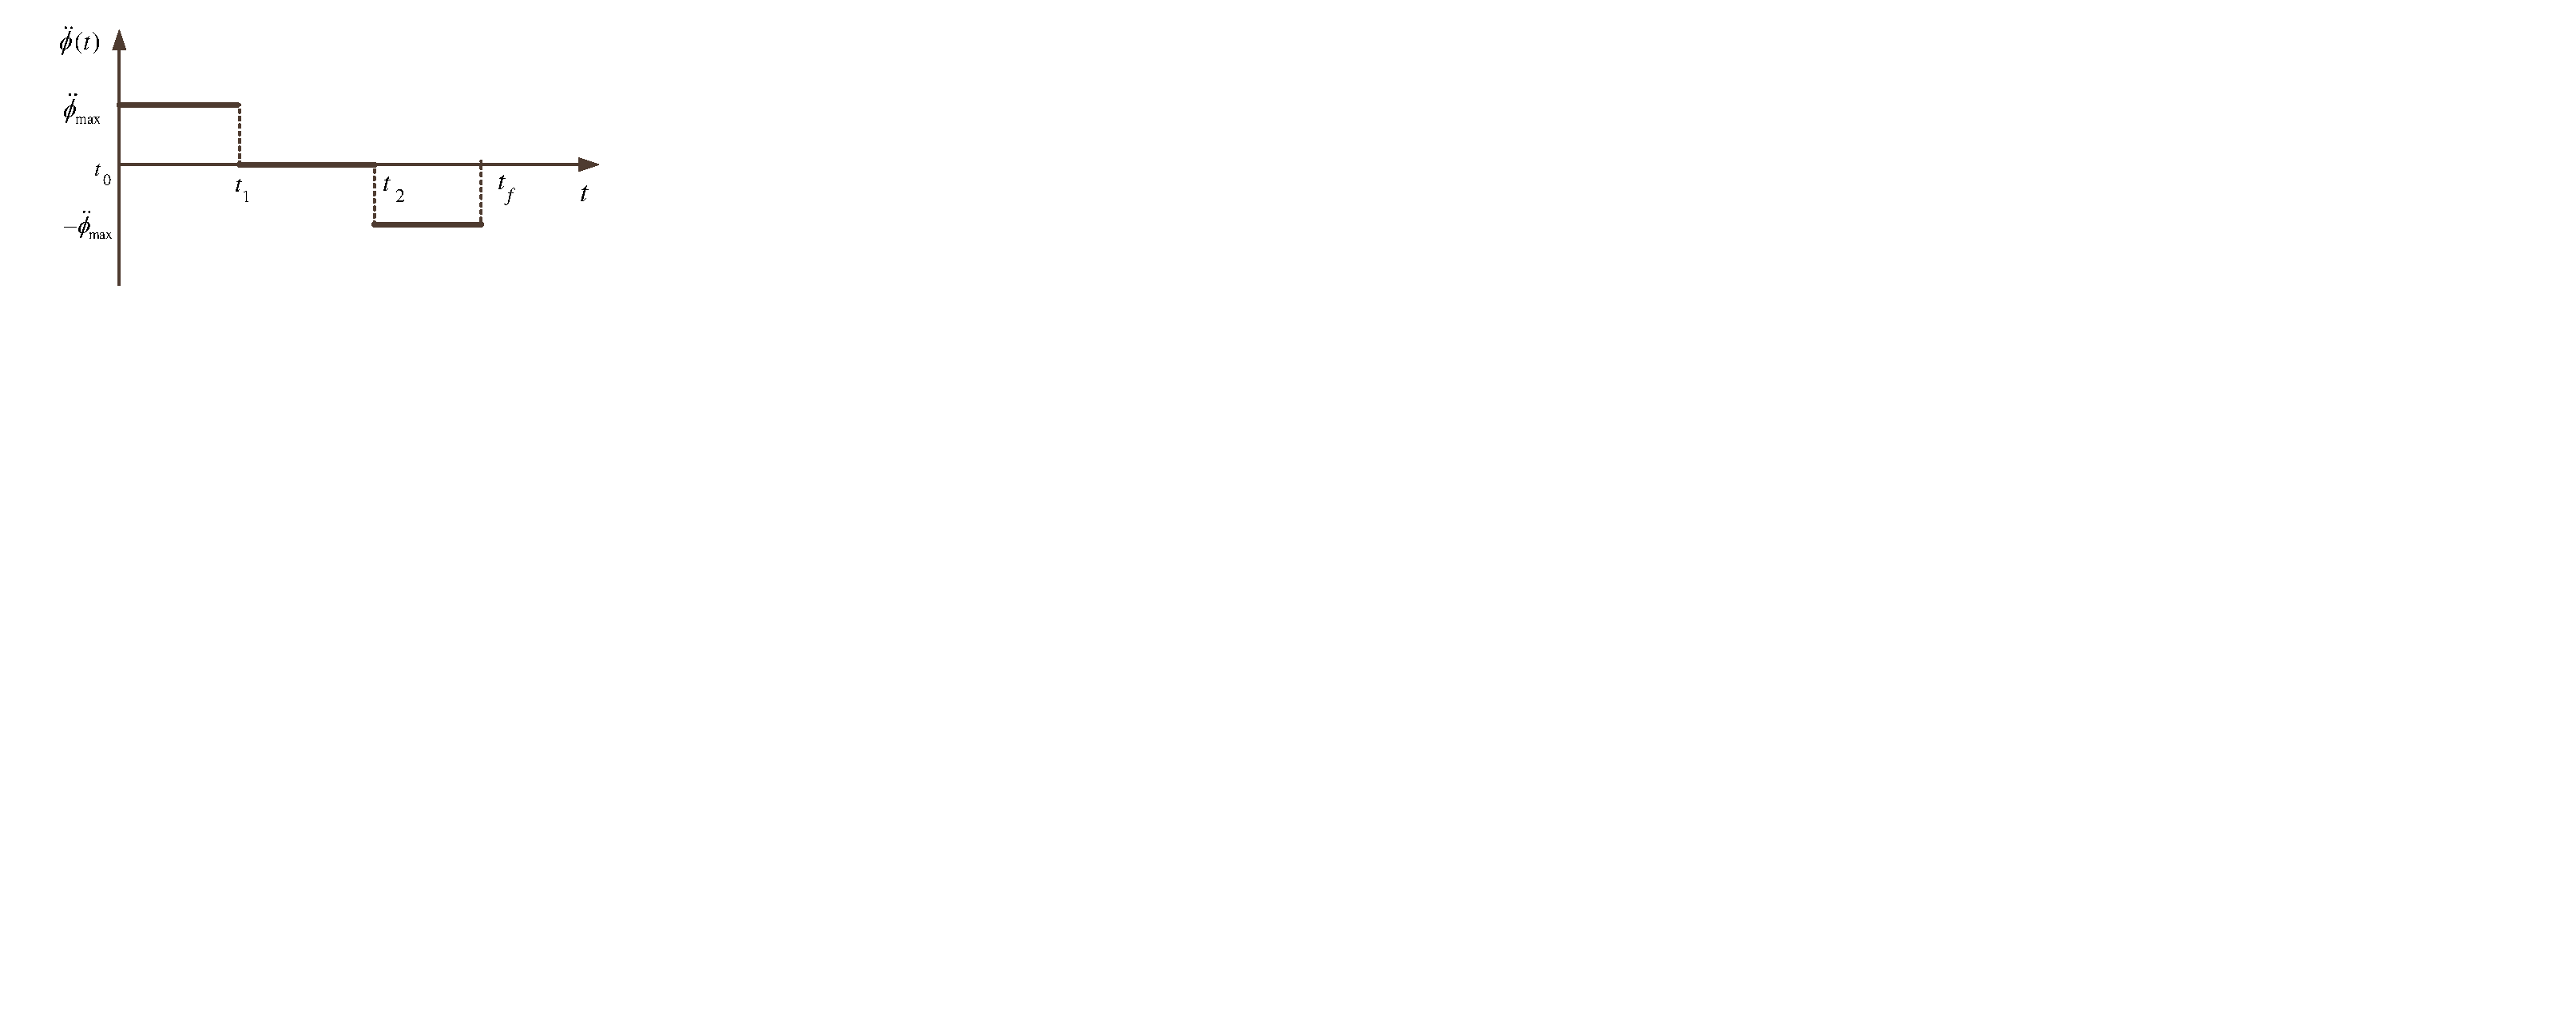
\includegraphics[width=1.5in]{./Figures/bang_off_bang}      
\end{center}
\end{minipage}
 \end{equation}
 \begin{itemize}
\item Angular velocity profile:
\end{itemize}
 \begin{equation}\label{phid_cons}
 \dot{\phi}(t)=\left\{
                \begin{array}{ll}
                \dot{\phi}_0+\ddot{\phi}_{max}(t-t_0)& when\  t_0\leq t\leq t_1,\\
                 \dot{\phi}_{max}& when\  t_1\leq t \leq t_2,\\
                 \dot{\phi}_{max}-\ddot{\phi}_{max}(t-t_2)& when \ t_2\leq t\leq t_f.
                \end{array}
              \right.
 \end{equation}
  \begin{itemize}
\item Angular position profile:
\end{itemize}
 \begin{equation}\label{phi_cons}
 \phi(t)=\left\{
                \begin{array}{ll}
                \dot{\phi}_0(t-t_0)+\frac{1}{2}\ddot{\phi}_{max}(t-t_0)^2& when\  t_0\leq t\leq t_1,\\
                \phi(t_1)+ \dot{\phi}_{max}(t-t_1)& when\  t_1\leq t \leq t_2,\\
                 \phi(t_2)+\dot{\phi}_{max}(t-t_2)-\frac{1}{2}\ddot{\phi}_{max}(t-t_2)^2& when \ t_2\leq t\leq t_f.
                \end{array}
              \right.
 \end{equation}
}
\end{block}
\end{frame}
%
%
%%-------------------------------------------------------------------------------------------------------------------------------------------------------------------
\begin{frame}{Computing Steering Profiles}

\begin{block}{ }
\begin{itemize}
\item Using the conditions, $\dot{\phi}(t_1)=\dot{\phi}_{max}$, $\dot{\phi}(t_f)=\dot{\phi}_f$, $\phi(t_f)=\phi_f$, we can determine switching times $t_1$, $t_2$, and final time $t_f$ as:
\end{itemize}
 \begin{equation}\label{t1cons}
t_1=t_0+\frac{\dot{\phi}_{max}-\dot{\phi}_0}{\ddot{\phi}_{max}},
 \end{equation}
 \begin{equation}\label{t2cons}
 \begin{split}
 t_2=&t_1+\frac{1}{\dot{\phi}_{max}}\Big[ \phi_f-\dot{\phi}_0(t_1-t_0)-\frac{1}{2}\ddot{\phi}_{max}(t_1-t_0)^2\\
 &-\frac{\dot{\phi}_{max}(\dot{\phi}_{max}-\dot{\phi}_f)}{\ddot{\phi}_{max}}+\frac{(\dot{\phi}_{max}-\dot{\phi}_f)^2}{2\ddot{\phi}_{max}} \Big],
 \end{split}
 \end{equation}
and
  \begin{equation}\label{tfcons}
 t_f=t_1+\frac{1}{\dot{\phi}_{max}}\Big[ \phi_f-\dot{\phi}_0(t_1-t_0)-\frac{1}{2}\ddot{\phi}_{max}(t_1-t_0)^2+\frac{(\dot{\phi}_{max}-\dot{\phi}_f)^2}{2\ddot{\phi}_{max}} \Big].
 \end{equation}
\end{block}
\end{frame}

%-------------------------------------------------------------------------------------------------------------------------------------------------------------------
\begin{frame}{Computing Steering Profiles}

\begin{block}{ }
\begin{itemize}
\item Steering profiles:
\begin{equation}
^Nq^D(t)=[e_x\sin\frac{\phi(t)}{2}, e_y\sin\frac{\phi(t)}{2}, e_z\sin\frac{\phi(t)}{2}, \cos\frac{\phi(t)}{2}]^T
\end{equation}
\begin{equation}
^N_G\omega^D(t)=\dot{\phi}(t)_G\hat{e}
\end{equation}
\begin{equation}
^N_G\alpha^D(t)=\ddot{\phi}(t)_G\hat{e}
\end{equation}
\end{itemize}
\end{block}
\end{frame}
%-------------------------------------------------------------------------------------------------------------------------------------------------------------------
\section{Numerical Simulations}
\begin{frame}{Numerical Simulations} 
	\begin{block}{Introduction}
		\begin{enumerate}
			\item Matlab was used to numerically simulate and examine the proposed algorithm. 
			\item The initial, final, and sun position vectors were randomized for each run. 
			\item Two cases shown in these slides - one in which the sun angle is greater than 0 from the slew plane, the other in which the sun vector lies directly on the slew plane. 
			\item Slew angles were found using the methods discussed in the description of the algorithm. 
		\end{enumerate}
	\end{block}
\end{frame}
%-------------------------------------------------------------------------------------------------------------------------------------------------------------------
%\begin{frame}{Numerical Simulations}
%\begin{block}{alpha $>$ 0}
%	
%	%				\newcommand*{\MyIndent}{\hspace*{0.5cm}}%
%	\begin{table}[H]
%		\centering
%		\caption{Slew Angles $\phi_1$, $\phi_2$, and $\phi_3$}
%		\begin{tabular}{llll}
%			\toprule
%			\midrule
%			$\phi$ & 1 & 2 & 3 \\
%			\midrule
%			Angle (rad) & 0.29 & 2.70 & 0.13 \\
%			Angle (deg) & 16.61 & 154.80 & 7.33 \\ 
%			\midrule
%			\bottomrule
%		\end{tabular}%
%		\label{tab:FOG_SF}%
%	\end{table}%
%	
%\end{block}
%\end{frame}
%%-------------------------------------------------------------------------------------------------------------------------------------------------------------------
\begin{frame}{Numerical Simulations}
	\begin{block}{$\alpha$ $>$ 0}
		\begin{figure}[H]
			\label{fig:phi1_phi2_phi3}
			\includegraphics[width=3in]{figures/alphaNot0/phi1_phi2_phi3.png}
			\caption{Attitude Profile of the Entire Slew}
		\end{figure}
	\end{block}
\end{frame}
%%-------------------------------------------------------------------------------------------------------------------------------------------------------------------
\begin{frame}{Numerical Simulations}
	\begin{block}{\alpha $>$ 0}
		
		\begin{figure}
			\centering
				\label{fig:ang_vel_phi_total}
					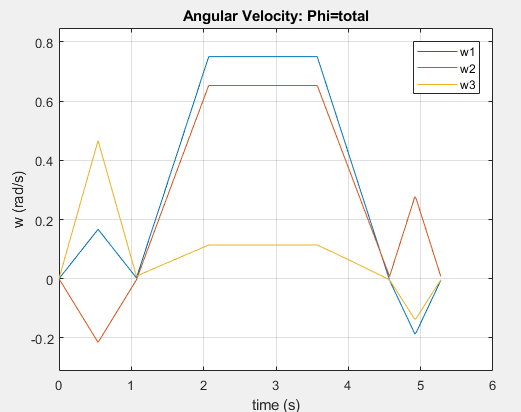
\includegraphics[width=3in]{figures/alphaNot0/ang_vel_phi_total.png}
				\caption{Angular Velocity in Spacecraft Frame}
		\end{figure}

%		\begin{figure}
%			\centering
%			\subfloat[caption 1]{{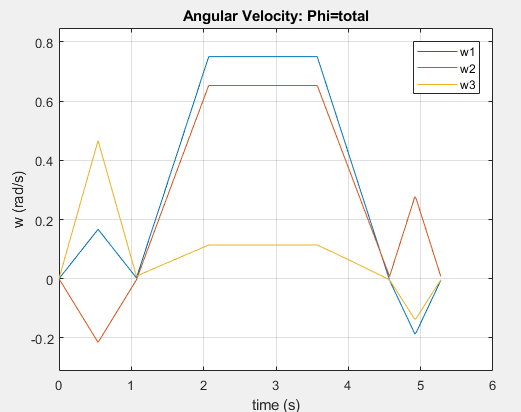
\includegraphics[width=1.5in]{figures/alphaNot0/ang_vel_phi_total.png} }}
%			\qquad
%			\subfloat[label 2]{{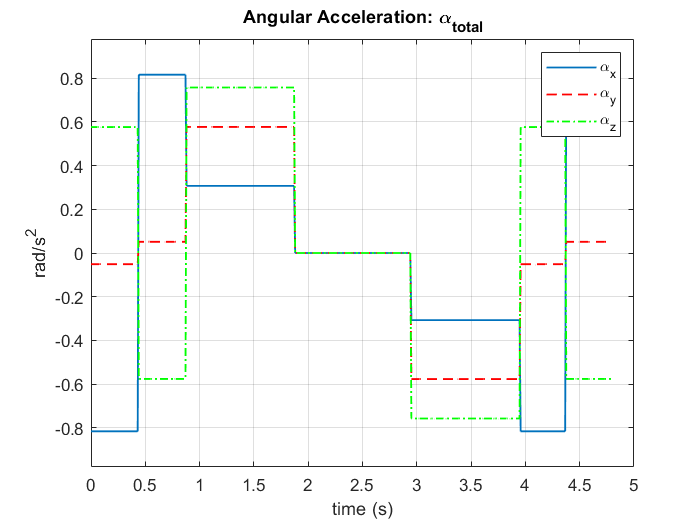
\includegraphics[width=1.5in]{figures/alphaNot0/ang_accel_total.png} }}
%			\caption{2 figures side by side} 
%			\label{fig:ex}
%		\end{figure}

	\end{block}
\end{frame}
%%-------------------------------------------------------------------------------------------------------------------------------------------------------------------
\begin{frame}{Numerical Simulations}
	\begin{block}{$\alpha$ $>$ 0}
		
		\begin{figure}[H]
			\label{fig:ang_accel_total}
			\begin{center}
				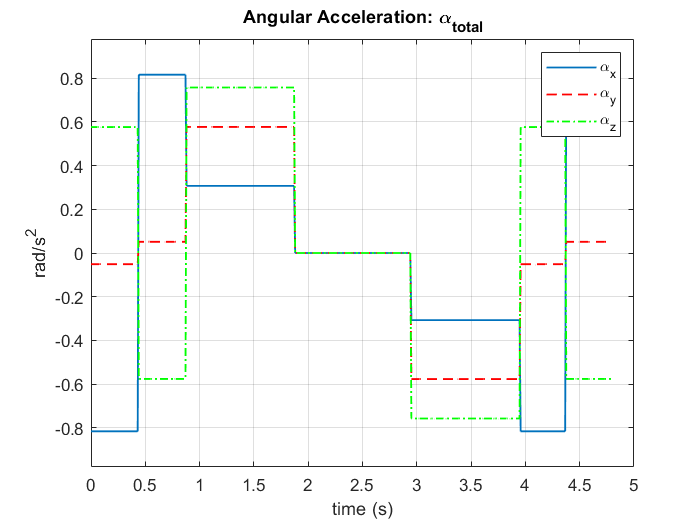
\includegraphics[width=3in]{figures/alphaNot0/ang_accel_total.png}
			\end{center}
			\caption{Angular Acceleration}
		\end{figure}
		
	\end{block}
\end{frame}
%%-------------------------------------------------------------------------------------------------------------------------------------------------------------------
\begin{frame}{Numerical Simulations}
\begin{block}{$\alpha$ $>$ 0}
	
	\begin{figure}[H]
		\label{fig:torque_total}
		\begin{center}
			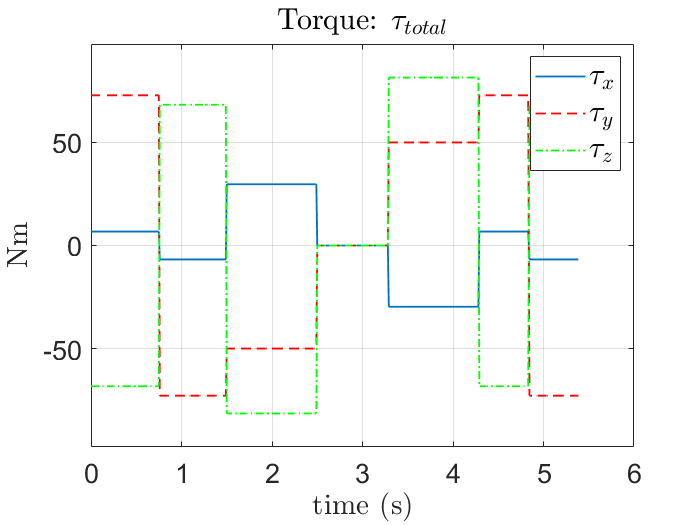
\includegraphics[width=3in]{figures/alphaNot0/torque_total.png}
		\end{center}
		\caption{Torque Applied from Actuator System}
	\end{figure}
	
\end{block}
\end{frame}
%%-------------------------------------------------------------------------------------------------------------------------------------------------------------------
\begin{frame}{Numerical Simulations}
	\begin{block}{$\alpha$ $>$ 0}
		
		\begin{figure}[H]
			\label{fig:quats_phi_total}
			\begin{center}
				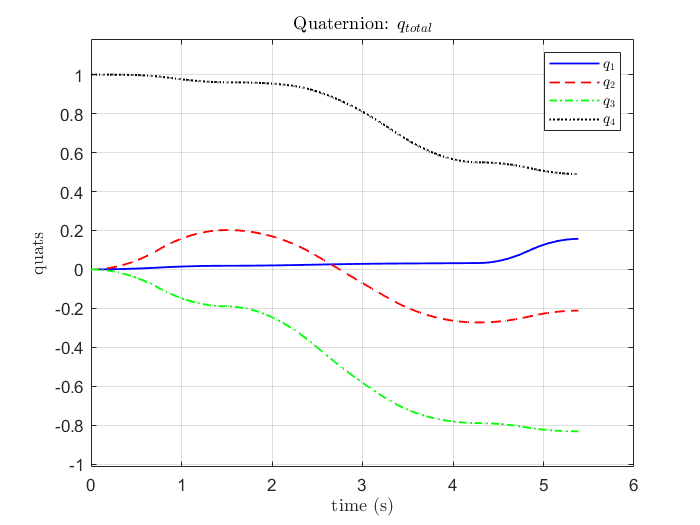
\includegraphics[width=3in]{figures/alphaNot0/quats_phi_total.png}
			\end{center}
			\caption{Quaternion Attitude}
		\end{figure}
		
		
	\end{block}
\end{frame}
\section{Summary and Conclusion}
\begin{frame}{Summary and Conclusion}
\begin{block}{}
	\begin{enumerate}
		\item Geometric approach for large-angle slew planning with pointing and actuator constraints 
		\item Assumed that initial and final attitudes, instrument boresight, and sun vector are known 
		\item Target-frame quaternions, angular velocities, and angular accelerations are derived base on the PMP 
		\item Limitation is for single sensitive-payload 
	\end{enumerate}
	
\end{block}
\end{frame}
%-------------------------------------------------------------------------------------------------------------------------------------------------------------------
\begin{frame}{Acknowledgments}
\begin{block}{}
	The research has been supported by Maxar Space Solutions (formerly Space Systems/Loral). The second author (Junette Hsin) would like to acknowledge Luke DeGalan for his useful comments. 
\end{block}
\end{frame}
%%%-------------------------------------------------------------------------------------------------------------------------------------------------------------------
%\begin{frame}
%\begin{block}{References}
%
%
%	\bibliographystyle{AAS_publication}   % Number the references.
%	\bibliography{references_SAA}   % Use references.bib to resolve the labels.
%
%\end{block}
%\end{frame}
%%-------------------------------------------------------------------------------------------------------------------------------------------------------------------
\section{Q\& A }
\begin{frame}
\begin{block}{}
\begin{center}
\Huge{Q \& A}
\end{center}
\end{block}
\end{frame}
%
%%%%%%%%%%%%%%%%%%%%%%%%%%%%%%%%%%%%%%%%%%%%%%%%%%%%%%%%%%%%%%%
%%-------------------------------------------------------------------------------------------------------------------------------------------------------------------
\begin{frame}
\begin{block}{}
\begin{center}
\Huge{Back-up Slides}
\end{center}
\end{block}
\end{frame}
%%-------------------------------------------------------------------------------------------------------------------------------------------------------------------
\begin{frame}
\begin{block}{}
\begin{center}
{\LARGE{Computing the Steering Profiles}}
\begin{center}
Case II: Single-Axis, Agile Slew Maneuver with Acceleration Constraint.
\end{center}
\end{center}
\end{block}
\end{frame}
%%-------------------------------------------------------------------------------------------------------------------------------------------------------------------
\begin{frame}
\begin{block}{ Single-Axis, Agile Slew Maneuver with Acceleration Constraint}
 {\bf Problem Statement:} \\ Consider the optimal control problem described by Eqs.(\ref{costfunction}), (\ref{system}), (\ref{Bcs}), and subject to control constraint
\begin{equation}
C_2: \ |u=\ddot{\phi}|\leq \ddot{\phi}_{max}.
\end{equation}
 {\bf Find:} $\phi(t)$, $\dot{\phi}(t)$, and $\ddot{\phi}(t)$.
 \end{block}
 \end{frame}
%
%%-------------------------------------------------------------------------------------------------------------------------------------------------------------------
\begin{frame}
\begin{block}{ Single-Axis, Agile Slew Maneuver with Acceleration Constraint}

\begin{itemize}
	\item Angular acceleration about the $\hat{e}$ axis:
\end{itemize}
\begin{equation}\label{alpha}
\ddot{\phi}(t)=\ddot{\phi}_{max}\mathbb{U}(t_0)- 2\ddot{\phi}_{max}\mathbb{U}(t-t_1)
\end{equation}

\begin{center}
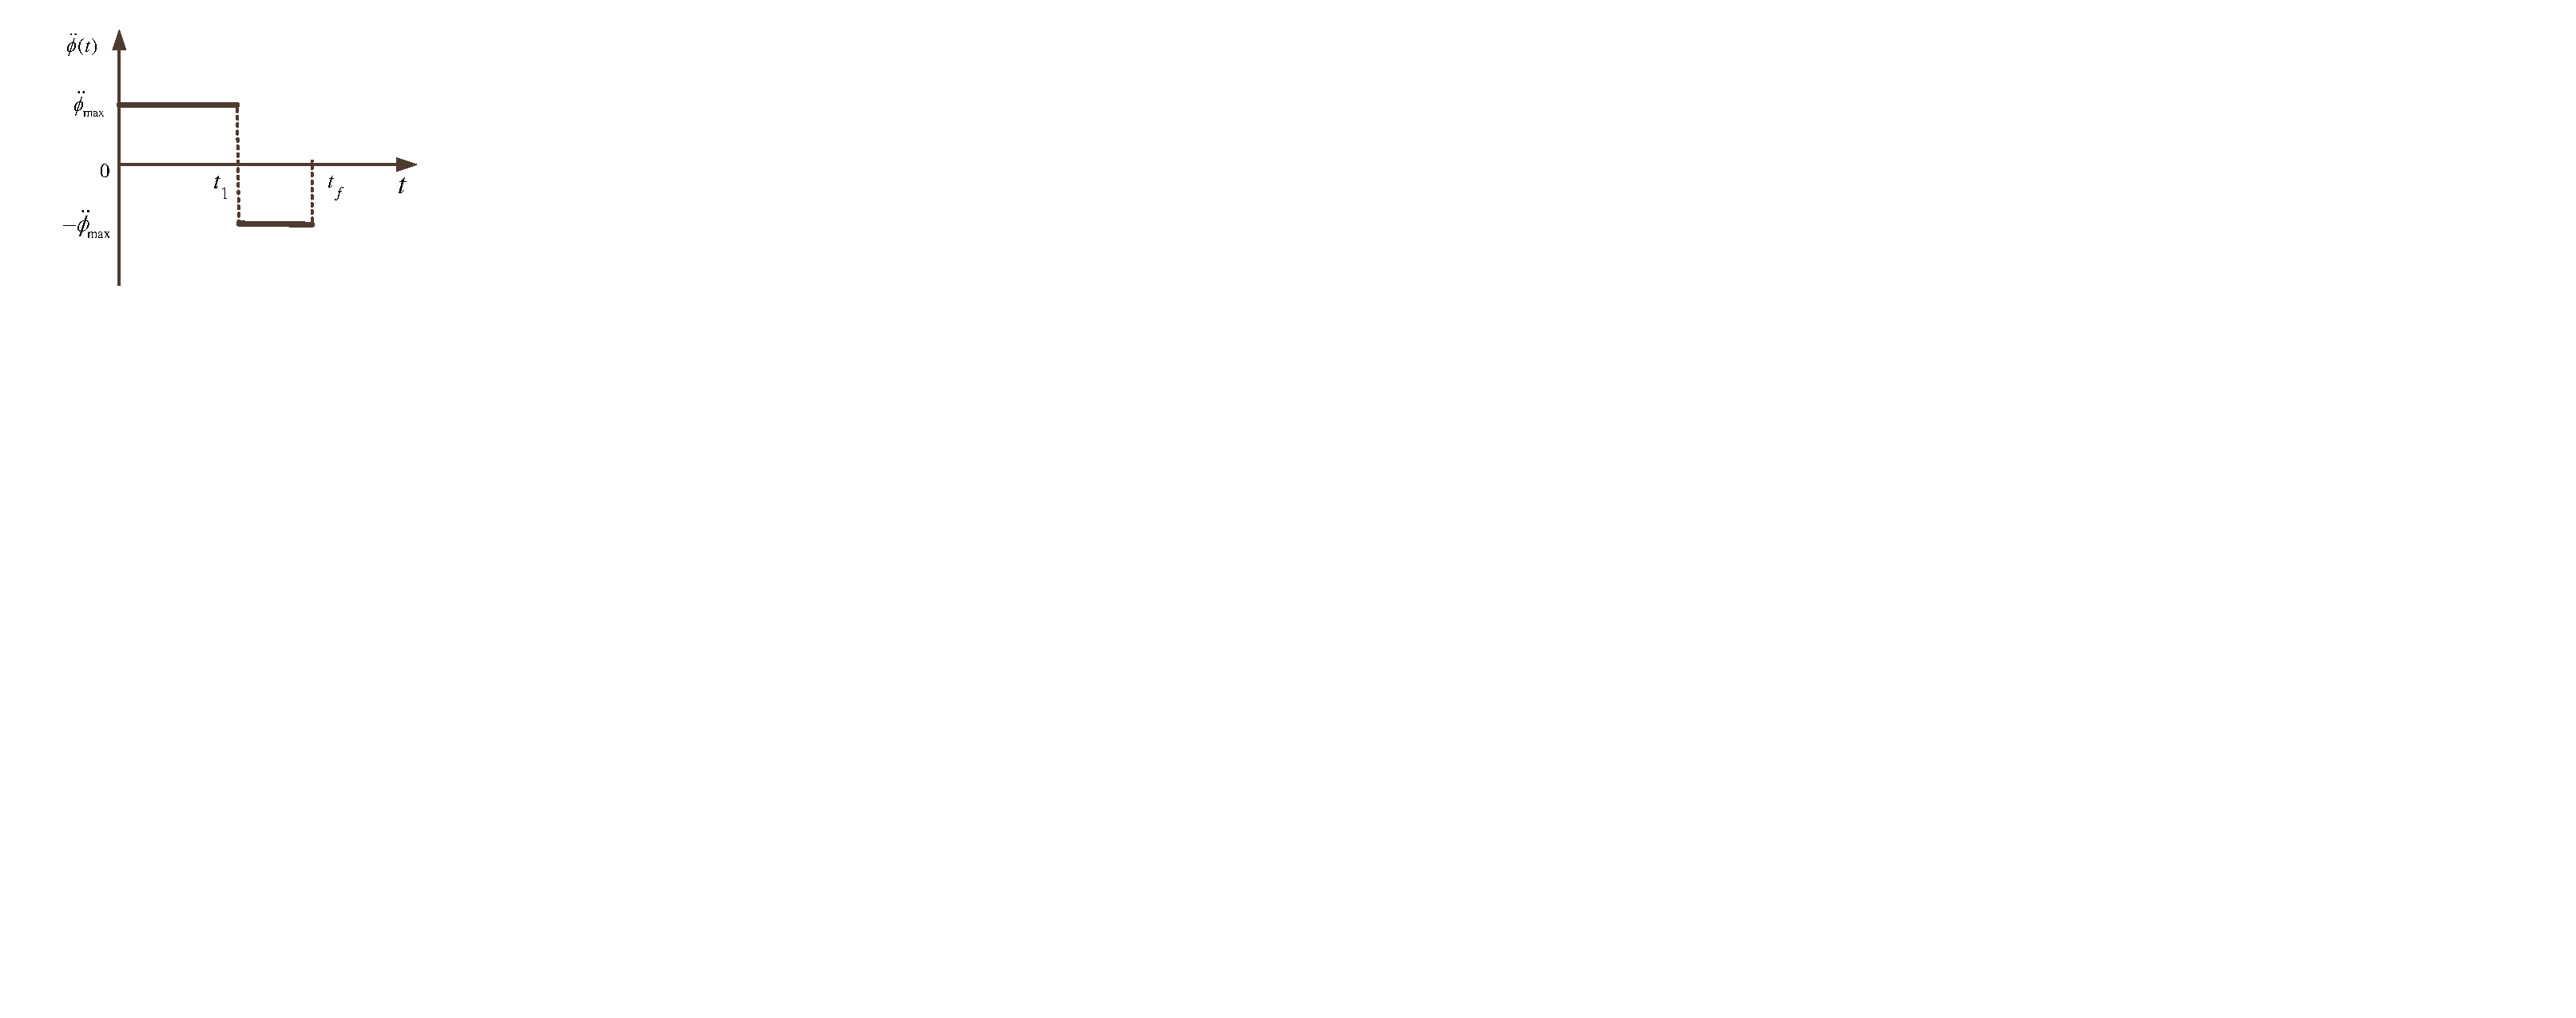
\includegraphics[width=2in]{./Figures/Bang_bang}      
\end{center}

where the switching and the final times are given by
\begin{equation}
t_1=t_0-\frac{\dot{\phi}_{0}}{\ddot{\phi}_{max}}+\frac{\sqrt{\ddot{\phi}_{max}^2(2\ddot{\phi}_{max}\phi_{f}+\dot{\phi}_{f}^2+\dot{\phi}_{0}^2)}}{\sqrt{2}\ddot{\phi}_{max}^2}
\end{equation}


\end{block}
\end{frame}
%%-------------------------------------------------------------------------------------------------------------------------------------------------------------------
\begin{frame}
\begin{block}{ Single-Axis, Agile Slew Maneuver with Acceleration Constraint}
and
\begin{equation}
t_f=t_0-\frac{\dot{\phi}_{f}+\dot{\phi}_{0}}{\ddot{\phi}_{max}}+\frac{\sqrt{2}\sqrt{\ddot{\phi}_{max}^2(2\ddot{\phi}_{max}\phi_{f}+\dot{\phi}_{ef}^2+\dot{\phi}_{0}^2)}}{\ddot{\phi}_{max}^2}
\end{equation}
\begin{itemize}
	\item Angular velocity about the $\hat{e}$ axis:
\end{itemize}
\begin{equation}\label{omega}
\dot{\phi}(t)=\dot{\phi}_{0}+\ddot{\phi}_{max}(t-t_0)\mathbb{U}(t_0)- 2\ddot{\phi}_{max}(t-t_1)\mathbb{U}(t-t_1)
\end{equation}
\begin{itemize}
	\item Angular position about the $\hat{e}$ axis:
\end{itemize}
\begin{equation}\label{phi}
\begin{split}
\phi(t)&=\dot{\phi}_{0}(t-t_0)+\ddot{\phi}_{max}\frac{(t-t_0)^2}{2}\mathbb{U}(t_0)\\
&- 2\ddot{\phi}_{max}\frac{(t-t_1)^2}{2}\mathbb{U}(t-t_1)
\end{split}
\end{equation}
\end{block}
\end{frame}

%-------------------------------------------------------------------------------------------------------------------------------------------------------------------
\begin{frame}{The Agile Sun-Avoidance Slew Maneuver}
\begin{block}{The First Slew Maneuver: \\ A single-axis nonrest-to-rest maneuver around the $\hat{e}$}

\begin{itemize}
\item The BCs: 
\end{itemize}
\begin{equation}\label{Bc1}
\dot{\phi}(t_0)=\dot{\phi}_{0},\phi(t_0)=0, \dot{\phi}(t_{f1})=0,\phi(t_{f1})=\phi_1.
\end{equation}

 The switching time, $t_{11}$, and minimum-time, $t_{f1}$, are
\begin{equation}\label{t11}
t_{11}=t_0-\frac{\dot{\phi}_0}{\ddot{\phi}_{max}}+\frac{\sqrt{\ddot{\phi}_{max}^2(2\ddot{\phi}_{max}\phi_1+\dot{\phi}_{0}^2)}}{\sqrt{2}\ddot{\phi}_{max}^2}
\end{equation}
\begin{equation}\label{tf1}
t_{f1}=t_0-\frac{\dot{\phi}_0}{\ddot{\phi}_{max}}+\frac{\sqrt{2\ddot{\phi}_{max}^2(2\ddot{\phi}_{max}\phi_1+\dot{\phi}_{0}^2)}}{\ddot{\phi}_{max}^2}
\end{equation}
The $\ddot{\phi}(t)$, $\dot{\phi}(t)$, and  $\phi(t)$,  can be found by substituting the boundary conditions given by (\ref{Bc1}) and $t_{11}$ and $t_{f1}$ in to Eqs. (\ref{alpha}), (\ref{omega}), and (\ref{phi}), respectively.
\end{block}
\end{frame}
%-------------------------------------------------------------------------------------------------------------------------------------------------------------------

\begin{frame}{The Agile Sun-Avoidance Slew Maneuver}
\begin{block}{The Second Slew Maneuver: A rest-to-rest maneuver around the sun vector}
\begin{itemize}
\item The BCs: 
\end{itemize}
\begin{equation}\label{Bc2}
\dot{\phi}(t_0)=0,\phi(t_0)=0, \dot{\phi}(t_{f2})=0,\phi(t_{f2})=\phi_2.
\end{equation}
 The switching time, $t_{12}$, and the minimum-time, $t_{f2}$, are
\begin{equation}\label{t21}
t_{12}=t_0-\frac{\sqrt{\phi_2}}{\ddot{\phi}_{max}}
\end{equation}
\begin{equation}\label{tf2}
t_{f2}=t_0-\frac{2\sqrt{\phi_2}}{\ddot{\phi}_{max}}
\end{equation}
The $\ddot{\phi}(t)$, $\dot{\phi}(t)$, and  $\phi(t)$,  can be found by substituting the boundary conditions given by (\ref{Bc2}) and $t_{12}$ and $t_{f2}$ in to Eqs. (\ref{alpha}), (\ref{omega}), and (\ref{phi}), respectively.
\end{block}
\end{frame}
%-------------------------------------------------------------------------------------------------------------------------------------------------------------------

\begin{frame}{The Agile Sun-Avoidance Slew Maneuver}
\begin{block}{The Third Slew Maneuver: A single-axis rest-to-nonrest maneuver around the $\hat{e}$}
\begin{itemize}
 \item The BCs: 
\end{itemize}
\begin{equation}\label{Bc3}
\dot{\phi}(t_0)=0,\phi(t_0)=0, \dot{\phi}(t_{f3})=\dot{\phi}_{f},\phi(t_{f3})=\phi_3.
\end{equation}
 The switching time, $t_{13}$, and the minimum-time, $t_{f3}$, are
\begin{equation}\label{t31}
t_{13}=t_0+\frac{\sqrt{\ddot{\phi}_{max}^2(2\ddot{\phi}_{max}\phi_3+\dot{\phi}_{f}^2)}}{\sqrt{2}\ddot{\phi}_{max}^2}
\end{equation}
\begin{equation}\label{tf3}
t_{f3}=t_0-\frac{\dot{\phi}_{f}}{\ddot{\phi}_{max}}+\frac{\sqrt{2\ddot{\phi}_{max}^2(2\ddot{\phi}_{max}\phi_3+\dot{\phi}_{f}^2)}}{\ddot{\phi}_{max}^2}
\end{equation}
The $\ddot{\phi}(t)$, $\dot{\phi}(t)$, and  $\phi(t)$,  can be found by substituting the boundary conditions given by (\ref{Bc3}) and $t_{13}$ and $t_{f3}$ in to Eqs. (\ref{alpha}), (\ref{omega}), and (\ref{phi}), respectively.
\end{block}
\end{frame}
%
%
%%-------------------------------------------------------------------------------------------------------------------------------------------------------------------
\begin{frame}{Computing Steering Profiles}

\begin{block}{ }
	\small{
		Using the Pontryagin's minimum principle (PMP), we derive the necessary conditions for the optimal solution as follows:
		\begin{enumerate}
			\item State Eqs.:
			\begin{equation}
			\left\{
			\begin{array}{l}
			\dot{x}_1=x_2, \\
			\dot{x}_2=u, \\
			\dot{x}_3=(x_2+\dot{\phi}_{max})^2\mathbb{U}(-x_2-\dot{\phi}_{max})+(\dot{\phi}_{max}-x_2)^2\mathbb{U}(x_2-\dot{\phi}_{max}),
			\end{array}
			\right.
			\end{equation}
			where the unit step function, $\mathbb{U}$, is defined as
			
			%		\begin{equation}
			%			\mathbb{U}(X)=\left\{
			%			                \begin{array}{lI}
			%			           1, & X > 0, \\
			%			           0, & X \leq 0.
			%			                \end{array}
			%			              \right.
			%		 \end{equation}
			
			\begin{equation}
			\mathbb{U}(X)=\left\{
			\begin{array}{l}
			1, X > 0, \\
			0, X \leq 0. \\
			\end{array}
			\right.
			\end{equation}
			
			Note:  ($x_3(t_0)=x_3(t_f)=0$ \& $x_3(t)\geq 0$ ) $\rightarrow x_3(t)=0, \forall t\in[t_0, t_f]. $  
			\item Hamiltonian:
			\begin{equation}
			\begin{split}
			\mathscr{H}=& 1+\lambda_1x_2+\lambda_2 u+\lambda_3\Big[(x_2+\dot{\phi}_{max})^2\mathbb{U}(-x_2-\dot{\phi}_{max})\\
			& (\dot{\phi}_{max}-x_2)^2\mathbb{U}(x_2-\dot{\phi}_{max})\Big]
			\end{split}
			\end{equation}
		\end{enumerate}
	}
	\seti
\end{block}
\end{frame}
%
%%-------------------------------------------------------------------------------------------------------------------------------------------------------------------
\begin{frame}{Computing Steering Profiles}

\begin{block}{ }
	\begin{enumerate}
		\conti
		\small{
			\item Costate Eqs.:
			\begin{equation}
			\left\{\begin{array}{l}
			\dot{\lambda}_1=-\frac{\partial{\mathscr{H}}}{\partial{x_1}}=0,\\
			\dot{\lambda}_2=-\frac{\partial{\mathscr{H}}}{\partial{x_2}}=-\lambda_1-2\lambda_3(x_2+\dot{\phi}_{max})\mathbb{U}(-x_2-\dot{\phi}_{max})\\
			+2\lambda_3(\dot{\phi}_{max}-x_2)\mathbb{U}(x_2-\dot{\phi}_{max}),\\
			\dot{\lambda}_3=-\frac{\partial{\mathscr{H}}}{\partial{x_3}}=0.\\
			\end{array}
			\right.
			\end{equation}
			\item Applying the Pontryagin's minimum principle (PMP),
			\begin{equation}
			u^*=arg \underset{u\in\mathcal{U}}{min} \mathscr{H},
			\end{equation}
			where $\mathcal{U}$ defines the domain of feasible controls. The optimal control can be determined as
			\begin{equation}
			u^*(t)=\left\{
			\begin{array}{I}
			\ddot{\phi}_{max}    \lambda_2<0,\\
			?    \lambda_2=0,\\
			-\ddot{\phi}_{max}    \lambda_2>0. \\
			\end{array}
			\right.
			\end{equation}
		}
	\end{enumerate}
	\seti
	This is a {\it singular arc} optimal control problem.
\end{block}
\end{frame}
%%
%%-------------------------------------------------------------------------------------------------------------------------------------------------------------------
\begin{frame}{Computing Steering Profiles}

\begin{block}{ }
	\begin{enumerate}
		\conti
		\item Determining the optimal control in the singular arc:
		\begin{equation}
		\frac{d^2}{dt^2}\Big(\frac{\partial \mathscr{H}}{\partial u}\Big)=\ddot{\lambda}_2=0\rightarrow \dot{x}_2=0\rightarrow u^*=0
		\end{equation}
		\item Checking the Generalized Legendre-Clebsch condition for optimality:
		\begin{equation}
		(-1)^2\frac{\partial}{\partial u}\Big[\frac{d^2}{dt^2}\Big(\frac{\partial \mathscr{H}}{\partial u}\Big)\Big]=1\geq 0
		\end{equation}
		\item The transversality condition:
		\begin{equation}
		\mathscr{H}|_{(*,t_f)}=0\  \text{and} \ \mathscr{H}\neq\mathscr{H}(t)\rightarrow \mathscr{H}=0, \forall t\in[t_0, t_f].
		\end{equation}
	\end{enumerate}
	\seti
\end{block}
\end{frame}
%%-------------------------------------------------------------------------------------------------------------------------------------------------------------------
%\begin{frame}{Numerical Simulations}
%	\begin{block}{alpha $=$ 0}
%		
%		\begin{table}[H]
%			\centering
%			\caption{Slew Angles $\phi_1$, $\phi_2$, and $\phi_3$}
%			\begin{tabular}{llll}
%				\toprule
%				\midrule
%				$\phi$ & 1 & 2 & 3 \\
%				\midrule
%				Angle (rad) & 0.02 & 3.14 & 0.00 \\
%				Angle (deg) & 10.80 & 180 & 0.00 \\ 
%				\midrule
%				\bottomrule
%			\end{tabular}%
%			\label{tab:FOG_SF}%
%		\end{table}% 
%		
%	\end{block}
%\end{frame}
%%-------------------------------------------------------------------------------------------------------------------------------------------------------------------
\begin{frame}{Numerical Simulations}
	\begin{block}{$\alpha$ $=$ 0}
		
		\begin{figure}[H]
			\label{fig:phi1_phi2_phi3_alpha0}
			\includegraphics[width=3in]{figures/alpha0/phi1_phi2_phi3.png}
			\caption{Attitude Profile of the Entire Slew}
		\end{figure}
		
	\end{block}
\end{frame}
%%-------------------------------------------------------------------------------------------------------------------------------------------------------------------
\begin{frame}{Numerical Simulations}
	\begin{block}{$\alpha$ $=$ 0}
		
		
		\begin{figure}[H]
			\label{fig:ang_vel_phi_total_alpha0}
			\begin{center}
				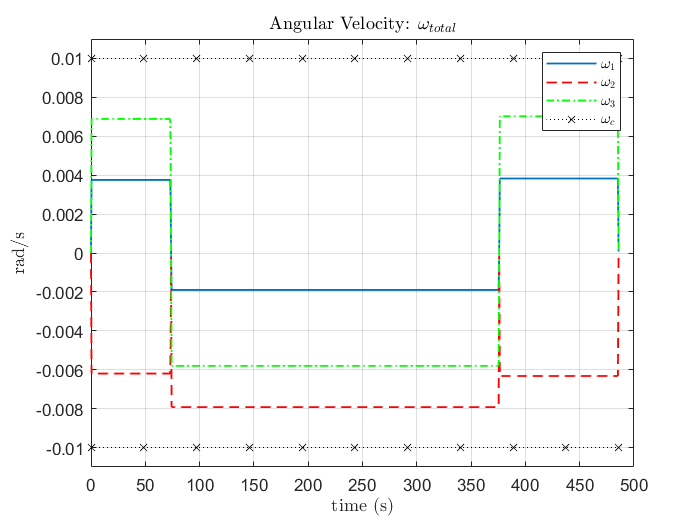
\includegraphics[width=3in]{figures/alpha0/ang_vel.png}
			\end{center}
			\caption{Angular Velocity in Spacecraft Frame}
		\end{figure}
		
	\end{block}
\end{frame}
%%-------------------------------------------------------------------------------------------------------------------------------------------------------------------
\begin{frame}{Numerical Simulations}
	\begin{block}{$\alpha$ $=$ 0}
		
		
		\begin{figure}[H]
			\label{fig:ang_accel_total_alpha0}
			\begin{center}
				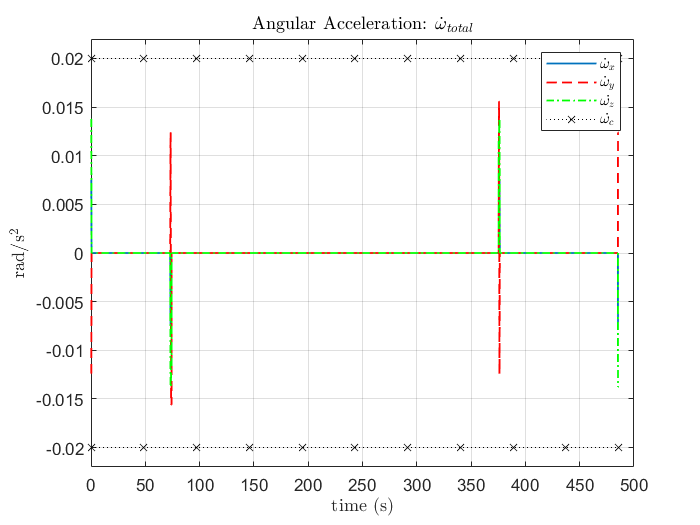
\includegraphics[width=3in]{figures/alpha0/ang_accel.png}
			\end{center}
			\caption{Angular Acceleration}
		\end{figure}
		
	\end{block}
\end{frame}
%%-------------------------------------------------------------------------------------------------------------------------------------------------------------------
\begin{frame}{Numerical Simulations}
	\begin{block}{$\alpha$ $=$ 0}
		
		\begin{figure}[H]
			\label{fig:torque_total_alpha0}
			\begin{center}
				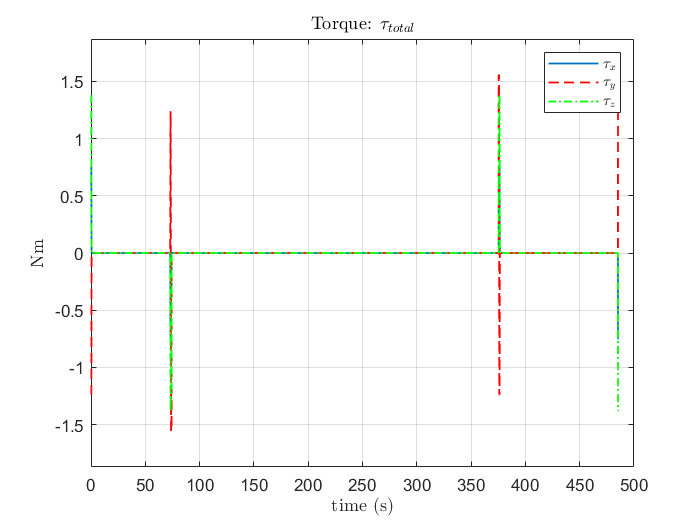
\includegraphics[width=3in]{figures/alpha0/torque.png}
			\end{center}
			\caption{Torque Applied from Actuator System}
		\end{figure}
		
	\end{block}
\end{frame}
%%-------------------------------------------------------------------------------------------------------------------------------------------------------------------
\begin{frame}{Numerical Simulations}
	\begin{block}{$\alpha$ $=$ 0}
		
		\begin{figure}[H]
			\label{fig:quats_phi_total_alpha0}
			\begin{center}
				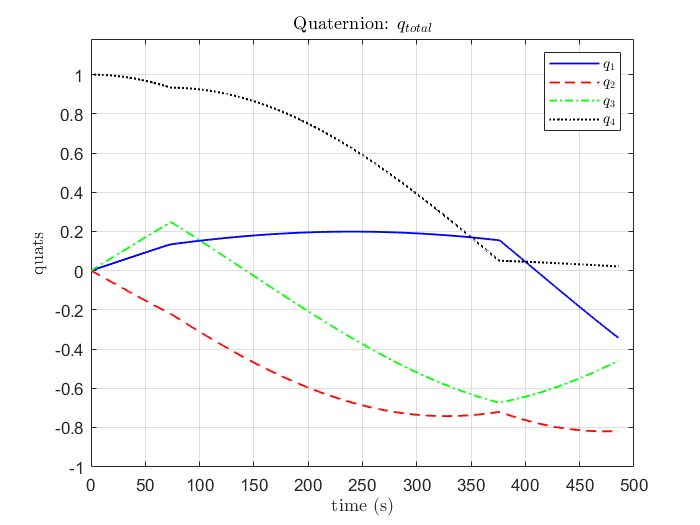
\includegraphics[width=3in]{figures/alpha0/quats.png}
			\end{center}
			\caption{Quaternion Attitude}
		\end{figure}
		
	\end{block}
\end{frame}
%%-------------------------------------------------------------------------------------------------------------------------------------------------------------------



\end{document}


